\documentclass[11pt]{report}

\usepackage[T1]{fontenc}
\usepackage[margin=1in]{geometry}
\usepackage[utf8]{inputenc}
\usepackage{apacite}
\usepackage{natbib, url}
\usepackage[english, french]{babel}
\usepackage{amsfonts, amsmath, amssymb}
\usepackage{amsthm}
\usepackage{color}
\usepackage{tabularx, booktabs} 
\usepackage{graphicx}
\graphicspath{ {images/} }
\usepackage{hyperref}
\usepackage{caption}
\usepackage{float}
\usepackage{listings}

\setlength{\abovecaptionskip}{2pt plus 0pt minus 0pt}

\setlength\parindent{0pt}

\frenchbsetup{%
    StandardItemizeEnv=true,       
    ThinSpaceInFrenchNumbers=true, 
    og=«, fg=»                     
  }
  
  \bibliographystyle{francais}


\newtheorem{theorem}{Théorème}[chapter]
\numberwithin{equation}{section}

\renewcommand{\listfigurename}{Liste des figures}

\begin{document}
% Tu gardes le strict minimum dans ton main (il sert juste à tout remettre ensemble pour compiler).
% Page titre dans un fichier séparé
% Page couverture du projet

\begin{titlepage}
    \begin{center}
        \vspace*{1cm}
        
        \Large
        \textbf{Modélisation statistique d'évènements extrêmes}
        
        \large
        \vspace{0.4cm}
        
        Application multivariée dynamique aux catastrophes naturelles de l'Océanie
 
        \vspace{3cm}
 
        \textit{Rapport soumis dans le cadre du cours ACT-2101 du} \\
        Baccalauréat en actuariat
 
        \vspace{1cm}
        
        \textit{Par}
 
        \textbf{Marc-Olivier Ricard}
        
        \vspace{1cm}
        
        \textit{Présenté à}
 
        \textbf{Marie-Pier Côté}
 
        \vfill
 
        
\includegraphics[width=0.3\textwidth]{Laval.PNG}
        
        \vspace{1.5cm}
 
        École d'actuariat\\
        Université Laval\\
        
        \vspace{0.5cm}
        
        Décembre 2019
 
    \end{center}
\end{titlepage}



\tableofcontents
\cleardoublepage
\listoftables
\listoffigures



% Résumé
\chapter*{Résumé}
\label{chap:résumé} 
\phantomsection\addcontentsline{toc}{chapter}{\nameref{chap:résumé}}


\chapter*{Remerciments}
\label{chap:merci} 
\phantomsection\addcontentsline{toc}{chapter}{\nameref{chap:merci}}

Je tiens à remercier Marie-Pier Côté pour la supervisation de mon projet de recherche et pour le temps qu'elle a investi dans celui-ci.

\chapter*{Introduction}
\label{chap:introduction} 
\phantomsection\addcontentsline{toc}{chapter}{\nameref{chap:introduction}}

L'objectif principal d'une analyse de valeur extrême est d'être capable de quantifier le comportement stochastique d'un processus à des niveaux exceptionnellement élevés ou bas. De plus, ce type d'analyse a souvent comme but d'estimer la probabilité de réalisation d'évènements qui sont encore plus extrêmes que n'importe quel évènement passé. La théorie des valeurs extrêmes rend ce genre d'extrapolation possible.



% Notions préliminaires

\chapter{Notions préliminaires}
\label{chap:notions} 

\section{Théorie classique des valeurs extrêmes}

Posons $M_n = \max\{X_1, \dots, X_n\}$, le maximum des n observations indépendantes et de distribution commune. Dans le cas où le comportement des $X_i$ serait connu, il serait facile d'obtenir le comportement exact de $M_n$, mais, en pratique, cette situation est très rare. Par contre, sous des hypothèses appropriées et pour ${n \to \infty}$, il est possible d'approximer le comportement de $M_n$ et d'obtenir une famille de modèles qui peuvent être ajustés avec les différentes valeurs observées. On appelle cette approche le paradigme des valeurs extrêmes. Il faut ensuite être en mesure d'estimer les différents paramètres du modèle, de quantifier l'incertitude, d'évaluer le modèle et finalement de maximiser l'utilisation de l'information disponible.\\

Dans cette section, on étudie le modèle qui s'intéresse au comportement statistique de $M_n$. Nous pourrions utiliser la distribution théorique:

\begin{equation}\label{eq:1.1.1}
\begin{split}
P\{M_n \le z\} &= P\{X_1 \le z, \dots, X_n \le z\} \\
              &= P\{X_1 \le z\} \times \dots \times P\{X_n \le z\} \\
              &= \{F(z)\}^n
\end{split}
\end{equation}

Par contre, en pratique, $F$ est inconnu et donc, cette approche n'est pas utile. Il serait possible d'estimer $F$ avec les valeurs observées, mais la moindre erreur dans l'estimation pourrait mener à une très grande erreur pour $F^n$. L'approche alternative est d'approximer directement $F^n$ avec seulement les valeurs extrêmes. Étant donné que la distribution de $M_n$ est dégénératrice à un certain point, nous normalisons $M_n$: 

\begin{equation}\label{eq:1.1.2}
M^*_n = \frac{M_n - b_n}{a_n}
\end{equation}

\begin{theorem}\label{theor:1.1}
S'il existe des séquences de constantes $\{a_n > 0\}$ et $\{b_n\}$ tel que $$P\Bigg\{\frac{M_n - b_n}{a_n} \le z \Bigg\}\to G(z), \ \ \  \text{quand} \ \ {n \to \infty}$$ où $G$ est une fonction de répartition non-dégénératrice. Alors, $G$ appartient à une des distributions de valeur extrême, soit les lois Gumbel, Fréchet et Weibull. Donc, peu importe la distribution ${F_X}_i$, les trois dernières lois sont les seules distributions limites pour $M^*_n$.
\end{theorem}

Malgré qu'il pourrait sembler logique de choisir une des trois distributions et d'estimer ses paramètres, cette piste possède deux faiblesses: une technique est nécessaire pour choisir la distribution la plus appropriée et dès que cette décision est prise, les inférences qui suivent présument que le bon choix a été fait. Une meilleure analyse est possible en combinant en une seule distribution les distributions Gumbel, Fréchet et Weibull:

\begin{equation}\label{eq:1.1.3}
\begin{gathered}
G(z) = \exp \Bigg\{ - \Big[ 1 +\xi\Big(\frac{z-\mu}{\sigma}\Big) \Big]^{-1/\xi}  \Bigg\}, \\
\{z: (1 + \xi(z- \mu)/\sigma) >0\},\ -\infty<\mu>\infty,\ \  \sigma>0,\ -\infty<\xi>\infty
\end{gathered}
\end{equation}

Ceci est la famille de distributions d'extremum généralisée (GEV). Comme on peut voir, le modèle possède trois paramètres: $\mu$ (paramètre de position), $\sigma$ (paramètre d'échelle), $\xi$ (paramètre de forme).\\

Si nous revenons au Théorème \ref{theor:1.1}, une autre difficulté est le fait que, en pratique, les constantes de normalisation $a_n$ et $b_n$ sont inconnus. Ce problème est facilement résolu: 

\begin{equation*}
\text{Nous savons déjà que} \ P\Bigg\{\frac{M_n - b_n}{a_n} \le z \Bigg\} \approx G(z), \ \ \text{quand} \ n\to\infty 
\end{equation*}

\begin{equation*}
\Rightarrow P\{M_n\le z\} \approx G\Bigg\{\frac{z- b_n}{a_n}\Bigg\} = G^*(z), 
\end{equation*}

où $G^*(z)$ est simplement un autre membre de la famille \textit{GEV}. Étant donné qu'en pratique, les paramètres doivent être estimés, ceci ne change rien au modèle proposé.\\

Tout ceci mène à une première méthodologie pour modéliser les valeurs extrêmes:

\begin{itemize}
\item Les données sont groupées en séquence de longueur $n$
\item Le maximum de chaque séquence est calculé
\item Une distribution \textit{GEV} est calibrée à ces maximums
\item La distribution peut être manipulée pour obtenir différentes statistiques
\end{itemize}

La distribution permet, par exemple, d'obtenir les très grands quantiles et ceux-ci sont obtenus comme ceci:
\begin{equation}\label{eq:1.1.4}
z_p =
\begin{cases}
\mu - \frac{\sigma}{\xi}\Big[1 - \{\log(1-p)\}^{-\xi}\Big], & \xi \ne 0 \\
\mu - \sigma\log\{-\log(1-p)\}, & \xi = 0
\end{cases}
\end{equation}
où:
\begin{itemize}
\item $G(z_p) = 1-p$
\item $z_p$ est le niveau de retour correspondant à la période de retour ${1}/{p}$
\item On s'attend à ce que le niveau $z_p$ soit dépassé en moyenne une fois chaque $1/p$ année.
\item Chaque année, le niveau $z_p$ est dépassé avec probabilité $p$
\end{itemize}

Nous pouvons également poser $y_p = -\log(1-p)$ pour obtenir:
\begin{equation}\label{eq:1.1.5}
z_p =
\begin{cases}
\mu - \frac{\sigma}{\xi}\Big[1 - {y_p}^{-\xi}\Big], & \xi \ne 0 \\
\mu - \sigma\log{y_p}, & \xi = 0
\end{cases}
\end{equation}
\\

Nous simplifions maintenant la notation en dénotant les maximums par $Z_1,\dots,Z_m$, on assume que ce sont des variables indépendantes d'une distribution \textit{GEV} dont il faut estimer les paramètres. À noter, que même si les $X_i$ sont dépendants, il peut être raisonnable d'assumer que les $Z_i$ sont indépendants.

La méthode la plus populaire pour l'estimation des paramètres est la méthode du maximum de vraisemblance. À noter, que si $\xi \le -0.5$,  il est fort probable qu'il sera impossible d'obtenir des estimateurs valides. Cependant, en pratique, cette situation est plutôt rare.\\

La log-vraisemblance va comme suit dans le cas où $\xi \ne 0$:

\begin{equation}\label{eq:1.1.6}
\begin{gathered}
\ell(\mu,\sigma,\xi) = -m\log\sigma - (1+{1/\xi})\sum_{i = 1}^{m}\log\Big[1+\xi\Big(\frac{z_i- \mu}{\sigma} \Big) \Big] - 
\sum_{i = 1}^{m}\Big[1+\xi\Big(\frac{z_i- \mu}{\sigma} \Big) \Big]^{-1/\xi},\\
1+\xi\Big(\frac{z_i- \mu}{\sigma}\Big) > 0,\ \ i=1,\dots,m
\end{gathered}
\end{equation}

Dans le cas où $\xi = 0$, il faut utiliser la limite Gumbel de la distribution:

\begin{equation}\label{eq:1.1.7}
\ell(\mu,\sigma) = -m\log\sigma - \sum_{i = 1}^{m}\Big(\frac{z_i- \mu}{\sigma} \Big)  -
\sum_{i = 1}^{m}\exp\Big[-\Big(\frac{z_i- \mu}{\sigma} \Big) \Big]
\end{equation}
\\

Après l'estimation des paramètres, nous pouvons estimer différents niveaux de retour:

\begin{equation}\label{eq:1.1.8}
\hat{z_p} = 
\begin{cases}
\hat\mu - \frac{\hat\sigma}{\hat\xi}\Big[1 - {y_p}^{-\hat\xi}\Big], & \hat\xi \ne 0 \\
\hat\mu - \hat\sigma\log{y_p}, & \hat\xi = 0
\end{cases}
\end{equation}

\begin{equation}\label{eq:1.1.9}
\text{Var}(\hat{z_p}) \approx \nabla z_p^T V \nabla z_p
\end{equation}
où $V$ correspond à la matrice variance-covariance de $(\hat\mu, \hat\sigma, \hat\xi)$ et

\begin{equation}\label{eq:1.1.10}
\begin{split}
\nabla z_p^T &= \Big[ \frac{\partial z_p}{\partial \mu}, \frac{\partial z_p}{\partial \sigma}, \frac{\partial z_p}{\partial \xi}\Big] \\
&= [1,\ -\xi^{-1}(1-y_p^{-\xi}),\ \sigma\xi^{-2}(1-y_p^{-\xi}) - \sigma\xi^{-1}y_p^{-\xi}\log y_p]\Bigg|_{(\hat\mu, \hat\sigma, \hat\xi)}
\end{split}
\end{equation}
\\

Même s'il est impossible de valider l'extrapolation faite par le modèle, on peut tout de même vérifier la qualité du modèle avec les données observées. Ces quatre graphiques sont utiles à cet effet:
\begin{itemize}
\item Graphique \textit{P-P}
\item Graphique \textit{Q-Q}
\item Graphique du niveau de retour
\item Histogramme des données avec la densité prédite par le modèle 
\end{itemize}


\section{Méthode par l'approche POT (\textit{Peaks over threshold})}

Un des inconvénients de la modélisation avec les maximums est qu'il y a potentiellement des données utiles qui ne sont pas utilisées étant donné que celles-ci ne sont pas le maximum de leur séquence, mais qui auraient pu être celui d'une autre séquence. La méthode présentée dans cette section fait une meilleure utilisation des données.\\

Soit $X_1, X_2,\dots$, une séquence de variables indépendantes, identiquement distribuées et avec fonction de répartition marginale $F$. Nous considérons comme évènements extrêmes ceux qui dépassent un certain seuil $u$. Le comportement stochastique d'un évènement extrême peut donc être décrit comme suit:

\begin{equation}\label{eq:1.2.1}
{\Pr{\{ X>u+y\ |\ X>u \}} = \frac{1-F(u+y)}{1- F(u)}}
\end{equation}

Si le comportement exact de $F$ était connu, la distribution de l'excès de seuil serait également connue. Cependant, en pratique, cette situation est rare et des approximations sont alors applicables lorsque $u$ est assez grand. \\

\begin{theorem}\label{theor:1.2}
Nous savons déjà que $\Pr\{ \max\{X_1,\dots,X_n\} \le z \}\approx G(z)$
où
\begin{equation*}
{G(z) = \exp \Bigg\{ - \Big[ 1 +\xi\Big(\frac{z-\mu}{\sigma}\Big) \Big]^{-1/\xi}  \Bigg\}}
\end{equation*}
Ensuite, pour $u$ assez grand, la fonction de répartition de $X-u\ |\ X>u$ est environ:
\begin{equation*}
H(y) = 1 - \Big(1+\frac{\xi y}{\tilde\sigma}\Big)^{-1/\xi},\ \{y:\ y>0\ \ \text{et}\ \ (1+ \xi y/\tilde{\sigma})>0 \} 
\end{equation*}
où
\begin{equation*}
{\tilde{\sigma} = \sigma + \xi(u-\mu)}
\end{equation*}
Il s'agit ici de la famille de distributions Pareto généralisée.
\end{theorem}

Nous avons donc comme théorème que si les maximums ont comme distribution approximative $G$, les excès de seuil ont comme distribution approximative un membre de la famille Pareto généralisée. De plus, les paramètres de $H$ sont uniquement déterminés par ceux de la distribution \textit{GEV}. $\xi$ conserve la même valeur, par exemple. La valeur de $n$ influence les paramètres de $G$, mais pas ceux de $H$.

\begin{proof}[Démonstration du théorème \ref{theor:1.2}]

\begin{equation*}
\begin{split}
F^n(z) \approx \exp \Bigg\{ - \Big[ 1 +\xi\Big(\frac{z-\mu}{\sigma}\Big) \Big]^{-1/\xi}  \Bigg\}\\
\Rightarrow n\log F(z) \approx - \Big[ 1 +\xi\Big(\frac{z-\mu}{\sigma}\Big) \Big]^{-1/\xi} 
\end{split}
\end{equation*}

Pour $n$ assez grand, un développement de Taylor donne:
\begin{equation*}
\begin{split}
\log F(z) \approx -(1-F(z))\\
\Rightarrow 1-F(u) \approx \frac{1}{n} \Big[ 1 +\xi\Big(\frac{u-\mu}{\sigma}\Big) \Big]^{-1/\xi}\\
\Rightarrow 1-F(u+y) \approx \frac{1}{n} \Big[ 1 +\xi\Big(\frac{u+y-\mu}{\sigma}\Big) \Big]^{-1/\xi}
\end{split}
\end{equation*}

\begin{equation*}
\begin{split}
\Rightarrow \Pr{\{ X>u+y\ |\ X>u \}} &\approx \frac{n^{-1}[1 + \xi(u+y-\mu)/\sigma]^{-1/\xi}}{n^{-1}[1 + \xi(u-\mu)/\sigma]^{-1/\xi}} \\
    &= \Bigg[ 1 + \frac{\xi(u+y-\mu)/\sigma}{1 + \xi(u-\mu)/\sigma}\Bigg]^{-1/\xi} \\
    &= \Bigg[1 + \frac{\xi y}{\tilde\sigma} \Bigg]^{-1/\xi},\ \ \tilde{\sigma} = \sigma + \xi(u - \mu)
\end{split}
\end{equation*}

\end{proof}


On propose le cadre suivant pour la modélisation de valeurs extrêmes: les données brutes représentent une séquence de valeurs indépendantes et identiquement distribuées $x_1,\dots,x_n$ et les valeurs extrêmes sont identifiées en définissant un seuil de grande valeur $u$. Les observations qui dépassent ce seuil sont définies par $x_{(1)},\dots,x_{(k)}$ et les excès de seuil par $y_j = x_{(j)} - u,\ j=1,\dots,k$. Ensuite, les $y_j$ sont reconnues comme des réalisations indépendantes d'une variable aléatoire dont la distribution peut être approximée par un membre de la famille Pareto généralisée.\\

Un des défis de cette démarche est le choix de la valeur de $u$, où il faut trouver une bonne balance entre la variance et le biais du modèle. La pratique standard est de choisir le plus petit $u$ possible qui respecte les hypothèses du modèle. Une première méthode est basée sur la moyenne de la distribution Pareto généralisée:

\begin{equation}\label{eq:1.2.2}
{\text{E}(Y) = \frac{\sigma}{1-\xi},\ \ \xi <1}
\end{equation}
Si la distribution est appropriée pour modéliser les excès d'un seuil $u_0$:
\begin{equation}\label{eq:1.2.3}
{\text{E}(X-u_0\ |\ X>u_0) = \frac{\sigma_{u_{0}}}{1- \xi}}
\end{equation}
où nous utilisons $\sigma_{u_{0}}$ pour le paramètre d'échelle des excès du seuil $u_0$. De plus, si la distribution est adéquate pour $u_0$, elle l'est également pour tous les seuils $u>u_0$ avec un changement approprié du paramètre d'échelle:

\begin{equation}\label{eq:1.2.4}
\begin{split}
\text{E}(X-u\ |\ X>u) &= {\frac{\sigma_u}{1-\xi}}\\
    &= {\frac{\sigma_{u_0} + \xi{(u-u_0)}}{1-\xi}}
\end{split}
\end{equation}
Donc, $\text{E}(X-u\ |\ X>u)$ est une fonction linéaire de $u$ et est également la moyenne des excès du seuil $u$. Cette moyenne peut être empiriquement approximée pour les données disponibles. Nous savons que ces approximés devraient changer linéairement avec $u$ quand la valeur de $u$ est appropriée pour le modèle Pareto généralisé. \\

Tout ceci mène finalement à la première procédure: nous considérons les points suivants:
\begin{equation}\label{eq:1.2.5}
\Bigg\{\Bigg(u,\ \frac{1}{n_u}\sum_{i=1}^{n_u}(x_{(i)} - u) \Bigg): u<x_{\text{max}}  \Bigg\}
\end{equation}

Cette séquence de points correspond au \textit{mean residual plot}. Après un seuil $u_0$ pour lequel la distribution Pareto généralisée fournie une approximation adéquate pour les excès, le graphique devrait être linéaire en $u$. Toutefois, il peut parfois être difficile d'interpréter ce type de graphique en pratique. \\

La deuxième méthode propose d'estimer le modèle pour différents seuils. Après un seuil $u_0$ pour lequel la distribution Pareto généralisée fournie une approximation adéquate pour les excès, les estimés du paramètre de forme $\xi$ devraient rester constants et les estimés de $\sigma_u$ devraient être linéaires en $u$ à moins que $\xi =0$, car $\sigma_u = \sigma_{u_0} + \xi(u - u_0)$. Nous pouvons également modifier le paramètre d'échelle de la distribution: $\sigma^* = \sigma_u - \xi u$. Avec cette paramétrisation, $\sigma^*$ et $\xi$ devraient rester constants au-delà de $u_0$. Nous pouvons donc tracer les graphiques de $\hat\sigma^*$ et $\hat\xi$ par rapport à $u$ et sélectionner $u_0$ comme la plus petite valeur of $u$ pour laquelle les estimés sont presque constants.\\ 

Après avoir choisi un seuil, les paramètres de la distribution Pareto généralisée peuvent être estimés avec la méthode du maximum de vraisemblance. Définissons $y_1,\dots,y_k$ comme les $k$ excès du seuil $u$. Pour $\xi \ne 0$, la log-vraisemblance est:
\begin{equation}\label{eq:1.2.6}
{\ell(\sigma, \xi) = -k\log\sigma - (1+1/\xi)\sum_{i=1}^{k}\log(1+\xi{y_i}/\sigma),\ \ (1+\xi{y_i}/\sigma) >0}
\end{equation}
Si $\xi =0$:
\begin{equation}\label{eq:1.2.7}
{\ell(\sigma) = -k\log\sigma - (1/\sigma)\sum_{i=1}^{k}y_i}
\end{equation}
Tout comme avec les maximums, des techniques numériques sont nécessaires pour la maximisation.\\

Pour les niveaux de retour, nous avons:
\begin{equation}\label{eq:1.2.8}
\begin{split}
{\Pr\{ X>x\ |\ X>u\} = \Big[ 1 + \xi \Big( \frac{x-u}{\sigma}\Big)\Big]^{-1/\xi}}\\
{\Rightarrow \Pr\{X>x\} = \zeta_u \Big[1 + \xi \Big( \frac{x-u}{\sigma}\Big)\Big]^{-1/\xi}}
\end{split}
\end{equation}
où $\zeta_u = \Pr\{X>u\}$. Ensuite, le niveau $x_m$ qui est dépassé en moyenne une fois chaque $m$ observations est obtenu comme suit:

\begin{equation}\label{eq:1.2.9}
\begin{split}
{\frac{1}{m} = \zeta_u \Big[1 + \xi \Big( \frac{x-u}{\sigma}\Big)\Big]^{-1/\xi}}\\
{\Rightarrow x_m = u + \frac{\sigma}{\xi} \Big[(m\zeta_u)^\xi -1\Big],\ \ x_m>u}
\end{split}
\end{equation}

Si $\xi =0$:
\begin{equation}\label{eq:1.2.10}
x_m = u + \sigma\log(m\zeta_u)
\end{equation}
\\

Il est souvent plus utile d'obtenir le niveau  qui est dépassé en moyenne une fois chaque $N$ années. S'il y a $n_y$ observations par années, le niveau de retour \textit{N-années} est défini comme suit:
\begin{equation}\label{eq:1.2.11}
z_N = u + \frac{\sigma}{\xi} \Big[(Nn_y \zeta_u)^\xi -1\Big]
\end{equation}
Si $\xi =0$:
\begin{equation}\label{eq:1.2.12}
z_N = u + \sigma\log(Nn_y\zeta_u)
\end{equation} 
\\

Pour estimer les niveaux de retour, il suffit de remplacer les paramètres par leur estimation. Pour $\xi$ et $\sigma$, il s'agit tout simplement de $\hat\xi$ et $\hat\sigma$ obtenus avec la méthode du maximum de vraisemblance et $\hat\zeta_u = k/n$, la proportion des données observées qui dépassent $u$. De plus, $\text{Var}(\hat\zeta_u) \approx \hat\zeta_u/(1- \hat\zeta_u)$, car $k \sim \text{Bin}(n,\zeta_u)$. \\

En appliquant la méthode delta:
\begin{equation}\label{eq:1.2.13}
\text{Var}(\hat{x}_m) \approx \nabla x^{\top}_m V \nabla x_m
\end{equation}
où $V$ correspond à la matrice variance-covariance de $(\hat\zeta_u,\hat\sigma, \hat\xi)$ et
\begin{equation}\label{eq:1.2.14}
\begin{split}
\nabla x^{\top}_m &= \Big[ \frac{\partial x_m}{\partial \zeta_u}, \frac{\partial x_m}{\partial \sigma}, \frac{\partial x_m}{\partial \xi}\Big] \\
&= \Big[\sigma^\xi \zeta^{\xi -1}_u,\ \xi^{-1} \{(m\zeta_u)^{\xi} -1\},\ -\sigma\xi^{-2}\{(m\zeta_u)^{\xi} -1\} + \sigma\xi^{-1}(m\zeta_u)^{\xi}\log(m\zeta_u)\Big]\Bigg|_{(\hat\zeta_u, \hat\sigma, \hat\xi)}
\end{split}
\end{equation}

De plus, pour la deuxième méthode de sélection de seuil, nous avons:
\begin{equation}\label{eq:1.2.15}
\text{Var}(\sigma^*) \approx \nabla \sigma^{*\top} V \nabla \sigma^*
\end{equation}
et 
\begin{equation}\label{eq:1.2.16}
\begin{split}
\nabla \sigma^{*\top} &= \Bigg[ \frac{\partial \sigma^*}{\partial \sigma_u}, \frac{\partial \sigma^*}{\partial \xi}\Bigg] \\
    &= [1, -u]
\end{split}
\end{equation}

Tout comme avec les maximums, ces quatre graphiques sont utiles pour la validation du modèle:

\begin{itemize}
\item Graphique \textit{P-P}
\item Graphique \textit{Q-Q}
\item Graphique du niveau de retour
\item Histogramme des données avec la densité prédite par le modèle 
\end{itemize}

Le graphique \textit{P-P} est constitué des points:
\begin{equation*}
\{ ((i/(k+1), \hat{H}(y_{(i)}));\ i=1,\dots,k\}
\end{equation*}
où
\begin{equation*}
\hat{H}(y) = 1 - \Bigg(1+\frac{\hat\xi y}{\hat\sigma}\Bigg)^{-1/\hat\xi}
\end{equation*}

Le graphique \textit{Q-Q} est constitué des points:
\begin{equation*}
\{(\hat{H}^{-1}(i/(k+1)), y_{(i)});\ i=1,\dots,k\}
\end{equation*}
où
\begin{equation*}
\hat{H}^{-1}(y) = u + \frac{\hat\sigma}{\hat\xi}\Big[y^{-\hat\xi}-1\Big]
\end{equation*}

Le graphique du niveau de retour est constitué des points:
\begin{equation*}
\{(m, \hat{x}_m)\}
\end{equation*}
où
\begin{equation*}
{\hat{x}_m = u + \frac{\hat\sigma}{\hat\xi} \Big[(m {\hat\zeta}_u)^{\hat\xi} -1\Big]}
\end{equation*}


\section{Modèles additifs généralisés et splines}
À compléter...

\section{Techniques de bootstrap}
À compléter...



% Article étudié
\chapter{Article étudié}
\label{chap:article}

\section{Introduction}
\label{sec:introar}
Dans le but d'aller au-delà des notions préliminaires du chapitre \ref{chap:notions}, un article en particuler a été étudié dans le cadre du projet de recherche. Plusieurs articles ont été brièvement explorés pour finalement choisir l'article qui répondait le plus aux bessoins du présent projet. L'article choisi (\cite{chavez2016extreme}) est tout de même récent, est de longueur et difficulté convenables et se penche sur un sujet spécifique intéressant en plus de fournir un implémentation en \textsf{R} de la méthode proposée. À noter que si le temps l'avait permis, \cite{thiombiano2017nonstationary} aurait également été un article intéressant à étudier. \\

L'article choisi présente une méthodologie dans laquelle la modélisation des valeurs extrêmes dépend de variables exogènes associées à la variable réponse qui est modélisée. Plus précisément, ce sont les paramètres du modèle de valeurs extrêmes choisi qui dépendront des covariables disponibles. C'est à dire que contrairement à ce qui a été vu aux sections \ref{sec:classique} et \ref{sec:pot} où les paramètres des modèles sont uniques étant donné qu'il sont obtenus par la méthode du maximum de vraisemblance avec l'ensemble des données, les auteurs proposent, ici, d'avoir des paramètres différents pour chaque niveaux de covariables. Cette approche vise à améliorer la calibration des lois aux données et du même coup rendre l'inférence plus crédible et précise. La méthode décrite propose de modéliser la fréquence de pertes avec un processus de Poisson non-homogène dont le paramètre dépend des covariables. Cette démarche implique l'utilisation des modèles additifs généralisés, des splines ainsi que la méthode du maximum de vraisemblance pénalisé. D'un autre côté, la sévérité est modélisée avec une distribution Pareto généralisée non-stationnaire dont les paramètre dépendent des variables exogènes. \footnote{L'article présente également la méthode avec la famille \textit{GEV}, mais brièvement.}. Ici, les splines de lissage ne peuvent pas être directement appliqués et l'article propose un algorithme basé sur les paramètres orthogonaux pour palier à la situation. Pour finir, les auteurs appliquent la méthodologie proposée à des données de pertes de risques opérationnels ainsi qu'à des données simulées pour valider la proposition.
\\

La méthodologie proposée dans l'article peut s'appliquer à plusieurs contextes et types de données qui respectent certains critères:
\begin{itemize}
\item Les données représentent des pertes aléatoires encourus à des temps aléatoires.
\item Le but de l'analyse est d'estimer la distribution de la perte globale à travers le temps.
\item Les données contiennent un nombre suffisant d'observations.
\item Les données contiennent des évènement (valeurs) extrêmes.
\item Les données contiennet des covariables significatives.
\end{itemize}

Il est important de noter que l'article utilise la méthodologie proposée avec des pertes, mais travailler avec des gains serait également possible. Même chose par rapport à des très grandes valeurs ou des très petites valeurs. Les critères mentionnés sont seulement générales et représentent une situation idéale. Quelqu'un pourrait très bien tenter d'appliquer la méthode même si un ou plusiers critères ne sont pas respectés et obtenir des résultats concluants. 
\\

À noter que les sections de l'article qui présentent les techniques de modélisation classiques ne seront pas discutés dans le présente section étant donné que l'ensemble de cette information peut être trouvé dans les sections \ref{sec:classique} et \ref{sec:pot}. La brève section sur l'approche dynamique avec les maximums ne sera également pas élaborée, car le focus de l'article ainsi que celui du chapitre \ref{chap:application} est vraiment l'approche \textit{POT}. 
\\

À noter également que le paramètre d'échelle $\sigma$ sera noté $\beta$ pour la suite des choses pour suivre la notation des auteurs de l'article.

\section{Approche dynamique de la théorie des valeurs extrêmes}

Comme mentionnée à la section \ref{sec:introar}, la nouvelle méthode proposée laisse les paramètres du modèle dépendent des covariables. Cette dépendance peut être paramétrique, non-paramétrique ou bien semi-paramétrique et elle peut également inclure des intéractions entre les variables. L'idée générale du modèle de dépendance entre les paramètres et les covariables peut être représenté par l'équation suivante:

\begin{equation}\label{eq:2.2.1}
g_k(\theta_k) = f_k(x) + h_k(x), \ \ k \in \{1, \dots, p \}
\end{equation}
où:
\begin{itemize}
\item $\theta$ est le vecteur des $p$ paramètres du modèle.
\item $g_k$ est une fonction de lien.
\item $f_k$ est la fonction pour les différents niveaux d'une variable catégorique.
\item $h_k$ est soit une fonction linéaire paramétrique ou bien une fonction lisse non-paramétrique de $t$.
\end{itemize}

 L'idée de dépendance entre les paramètres du modèle et des covariables a déjà élaborée dans \cite{coles2001introduction}, ce qui est réellement nouveau dans l'approche proposée est la dépendance semi-paramétrique avec les splines de lissage. \\
 
 Ensuite, le vecteur des paramètres du modèle $\theta$ peut être estimé en maximisant la log-vraisemblance pénalisée:
 \begin{equation}\label{eq:2.2.2}
 \ell(\theta; \cdot) - \sum_{k=1}^{p}\Big(\gamma_k \int_A h''_k(t)^2 \,dt\Big)
 \end{equation}
 où $ \ell(\theta; \cdot)$ est tout simplement la log-vraisemblance du modèle, \textit{POT} ici. Le terme de pénalité est une technique répandue qui a pour but d'éviter du surapprentissage des données. À noter que plus $\gamma_k$ est grand, plus la courbe obtenue est lisse et vice-versa. 
 \\
 
On assume que le nombre d'excès du seuil $u$ sélectionné suit un processus de Poisson non-homogène avec comme taux:
 \begin{equation}\label{eq:2.2.3}
 \lambda = \lambda(x, t) = \exp(f_\lambda(x) + f_\lambda(t))
  \end{equation}
  où $f_\lambda$ est une fonction pour les différents niveaux d'une variable catégorique $x$ et $h_\lambda$ est une fonction générale qui ne dépend pas de paramètres spécifiques comme c'est le cas pour $f_\lambda$. Ensuite, l'application d'un modèle additif généralisé mène à un estimé $\hat\lambda$ qui sera utile pour le reste de la modélisation. Cette étape peut être complétée avec l'aide du logiciel \textsf{R} et du paquetage \texttt{mgcv}.
  \\  
  
  L'approche est très semblable à l'équation \ref{eq:2.2.3} pour ce qui est de la modélisation de la sévérité de la perte. Cependant, une étape supplémentaire est nécessaire pour s'assurer que les procédures de calibration des paramètres $\xi$ et $\beta$ aux données convergent. Pour ce faire, il faut absolument que ces deux paramètres soient orthogonaux par rapport à l'information de Fisher. De ce fait, $\beta$ est reparamétrisé comme suit:
 \begin{equation}\label{eq:2.2.4}
 \begin{split}
  \nu = \log((1+\xi)\beta) \ \ \xi > -1
  \Rightarrow \beta = \frac{\exp(\nu)}{1+\xi}
  \end{split}
  \end{equation}
ce qui est orthognal à $\xi$. Voir \cite{cox1987parameter} pour plus de détails. En suit la log-vraisemblance reparamétrisée:
 \begin{equation}\label{eq:2.2.5}
 \ell(\theta; \cdot) \longrightarrow \ell^r(\xi, \nu; y) = \ell\Big(\xi, \frac{\exp(\nu)}{1+\xi}; y\Big)
 \end{equation}
où Y représente le vecteur des excès de seuil $u$. 
\\

Dans la même ordre d'idée que pour $\lambda$, on définit $\xi$ et $\nu$ comme suit:
\begin{equation}\label{eq:2.2.6}
 \xi = \xi(x, t) = f_\xi(x) + f_\xi(t)
\end{equation}
  
 \begin{equation}\label{eq:2.2.7}
 \nu = \nu(x, t) = f_\nu(x) + f_\nu(t)
 \end{equation}
 
  \begin{equation}\label{eq:2.2.8}
  \Rightarrow \beta = \beta(x, t) =  \frac{\exp(\nu(x,t))}{1+\xi(x,t)}
 \end{equation}

Les équations \ref{eq:2.2.6} et \ref{eq:2.2.7} sont donc celles qui seront estimées avec les excès de seuil disponibles pour être en mesure d'obtenir $\hat\xi$ et $\hat\beta$. Ces estimateurs sont donc des estimateurs basés sur les estimateurs $\hat{f}_\xi, \hat{h}_\xi, \hat{f}_\nu$ et$ \hat{h}_\nu$. Ces derniers estimateurs sont obtenus à partir des vecteurs observés $z_i = (t_i, x_i, {y_t}_{i})$ où:
\begin{itemize}
\item $i \in \{1, \dots, n\}$.
\item $0 \leq t_1 \le \cdots \le t_n \leq T$ représente les temps d'excès de seuil.
\item $x_i$ représente le vecteur des covariables.
\item ${y_t}_{i}$ représente les réalisations de la variable aléatoire ${Y_t}_{i}$.
\item ${Y_t}_{i}$ représente les excès de seuil $u$.
\end{itemize}

Contrairement à la méthode présentée pour la fréquence (équation \ref{eq:2.2.3}), un modèle additif généralisé n'est pas suffissant ici et un algorithme est donc développé pour être en mesure d'obtenir les paramètres estimés. Pour être en mesure d'ajuster des fonctions $h_\xi$ et $h_\nu$ qui sont assez lisses ont vecteurs observés $z_i$, la log-vraisemblance de l'équation \ref{eq:2.2.2} est utilisée:
 \begin{equation}\label{eq:2.2.9}
\ell^p({f}_\xi, {h}_\xi, {f}_\nu, {h}_\nu; z_1, \dots, z_n) =  \ell^r(\xi, \nu; y) - \gamma_\xi \int_{0}^{T} h''_\xi(t)^2 \,dt - \gamma_\nu\int_{0}^{T}  h''_\nu(t)^2 \,dt 
\end{equation}
où 
\begin{itemize}
\item $ \gamma_\xi,  \gamma_\nu \geq 0$ sont les paramètres de lissage. 
\item $y=({y_t}_{1}, \dots, {y_t}_{n})$.
\item $\ell^r(\xi, \nu; y) = \sum_{i=1}^{n} \ell^r(\xi_i, \nu_i; {y_t}_{i}) = \sum_{i=1}^{n} \ell^r(\xi_i,\frac{\exp(\nu_i)}{1+\xi_i} ; y_i)$
\end{itemize}


En combinant les conditions énumérés à la section \ref{sec:gam} et \cite[p.~13]{green1993nonparametric}, pour une spline naturelle cubique $h$ ayant comme noeuds $s_1, \dots, s_m$:
\begin{equation}\label{eq:2.2.10}
\int_{0}^{T} h''(t)^2dt = h^{\top} K h
\end{equation}
où 
\begin{itemize}
\item $h=({h_s}_1, \dots, {h_s}_n) = (h(s_1), \dots, h(s_n))$,
\item $K$ est une matrice symétrique de $m$ colonnes de rang $m-2$ qui dépend des noeuds $s_1, \dots, s_m$
\end{itemize}

Du coup, l'équation \ref{eq:2.2.9} peut être réécrite comme suit:
\begin{equation}\label{eq:2.2.10}
\ell^p({f}_\xi, {h}_\xi, {f}_\nu, {h}_\nu; z_1, \dots, z_n) =  \ell^r(\xi, \nu; y) - \gamma_\xi  {h_\xi}^{\top} K {h_\xi} - \gamma_\nu  {h_\nu}^{\top} K {h_\nu}
\end{equation}

C'est avec l'obtention de cette formule que devient possible le développement d'un algorithme permettant d'obtenir $\hat\xi$ et $\hat\beta$.  Des intervalles de confiance pour les paramètres sont également obtenus avec l'aide d'une technique de bootstrap. Cet algorithme est présenté à la section \ref{sec:algos}. 
\\

Après avoir obtenu les paramètres estimés du modèle utilisé et avant d'appliquer tout genre d'inférence avec le modèle obtenu, il est nécessaire d'évaluer la qualité de celui-ci. La méthode proposée ici repose sur le fait que si les excès ${Y_t}_{i}$ suivent une distribution Pareto généralisée avec comme paramètre $\xi$ et $\beta$, $R_i = 1 - G_{\xi_i, \beta_i} ({Y_t}_{i}), \ i \in \{1, \dots, n\}$ forme approximativement un échantillon aléatoire d'une loi uniforme $U(0,1)$. Ainsi, il est possible de vérifier si les valeurs $r_i$ se comportent comme des variables aléatoires indépendantes suivant une loi exponentielle standard où
\begin{equation}\label{eq:2.2.11}
r_i = -\log(1 - G_{\hat\xi_i, \hat\beta_i}({y_t}_{i})), \ \ i \in \{1, \dots, n\}
\end{equation}

Finalement, lorsque tous les paramètres sont obtenus et que l'adéquation du modèle est validé, l'inférence et plus particulièrement le calcul de mesures de risques pour des covariables et un point dans le temps en particulier est possible:
\begin{equation}\label{eq:2.2.12}
\widehat{\text{VaR}_\alpha} = u + \frac{\hat\beta}{\hat\xi} \Bigg(\Bigg( \frac{1-\alpha}{\hat\lambda/n'}\Bigg)^{-\hat\xi} -1 \Bigg)
\end{equation}

\begin{equation}\label{eq:2.2.13}
\widehat{\text{ES}_\alpha} =
\begin{cases}
\frac{\widehat{\text{VaR}_\alpha} + \hat\beta + u\hat\xi}{1-\hat\xi}, & \hat{\xi} \in (0,1) \\
\infty, & \hat\xi 	\ge 1
\end{cases}
\end{equation}
où $n' = n'(x,t)$ représente le nombre total de pertes pour les covariables $x$ et pour le temps $t$. Cependant, en pratique, il est plus utile de modéliser directement $\rho = \rho(x, t) = \lambda(x,t)/n'(x, t)$ qui représente le taux d'excès de seuil pour $x$ et $t$ avec une régression logistique. Des intervalles de confiance sont obtenus pour les mesures de risque avec une technique de bootstrap.
\\

Un dernier court point à couvrir est le choix du paramètre de lissage souvent reconnu comme le nombre de degrés de liberté. L'utilisation du critère d'information d'Akaike (AIC) est la technique proposée par les auteurs.
\begin{equation}\label{eq:2.2.14}
\text{AIC} \propto -2 \ell(\theta; \cdot) + 2\text{Df}
\end{equation}

\section{Application à des données réelles}
La présente section discute des fait saillants de l'application de la méthodologie à des données réelles faite par les auteurs de l'article. Voir \cite{chavez2016extreme} pour de plus amples détails.



\section{Discussion}

\section{Algorithmes}
\label{sec:algos}



%% Application à des données réelles
% le Sweaveopt


\chapter{Application à des données réelles}
\label{chap:application} 

\section{Analyse de données}

Pour mettre en application l'approche proposée par \cite{chavez2016extreme}, deux jeux de données du paquetage \texttt{CASdatasets} sont utilisés. Soit \texttt{auscathist} et \texttt{nzcathist}. Ces données représentent respectivement l'historique des catastrophes naturelles pour l'Australie ainsi que pour la Nouvelle-Zélande. Les deux jeux de données contiennent également différentes statistiques de ces catastrophes. Voici une liste des variables disponibles:
\begin{itemize}
\item \texttt{Year}: l'année d'occurence de la catastrophe.
\item \texttt{Quarter}: le trimestre d'occurence de la catastrophne.
\item \texttt{Date}: la date d'occurence complète de la catastrophe.
\item \texttt{FirstDay}: la date de la première journée d'occurence de la catastrophe.
\item \texttt{LastDay}: la date de la dernière journée de la catastrophe (seulement disponible pour l'Australie).
\item \texttt{Event}: une description de la catastrophe.
\item \texttt{Type}: le type de catastrophe.
\item \texttt{Location}: une description du lieu de la catastrophe.
\item \texttt{OriginalCost}: coût original de la catastrophe en millions de \textit{AUD} ou \textit{NZD}.
\item \texttt{NormCost2011}: coût normalisé en millions de dollars de 2011 (inflation, richesse et population).
\item \texttt{NormCost2014}: coût normalisé en millions de dollars de 2014 (inflation, richesse et population).
\end{itemize}
\

Les tables \ref{tab:3.1} et \ref{tab:3.2} contiennent un résumé statistique des données australiennes. Les tables \ref{tab:3.3} et \ref{tab:3.4} contiennent le même type de résumé pour la Nouvelle-Zélande.


% latex table generated in R 3.6.1 by xtable 1.8-4 package
% Mon Dec  2 15:08:45 2019
\begin{table}[ht]
\centering
\begin{tabular}{cccccccc}
  \hline
 & Mean & Std.Dev & Min & Median & Max & N.Valid & Pct.Valid \\ 
  \hline
NormCost2011 & 254 & 589 & 2 & 66 & 4296 & 190 & 92 \\ 
  NormCost2014 & 288 & 639 & 2 & 77 & 4606 & 206 & 100 \\ 
  OriginalCost & 104 & 295 & 1 & 15 & 2388 & 206 & 100 \\ 
  Quarter & 2 & 1 & 1 & 2 & 4 & 206 & 100 \\ 
  Year & 1995 & 12 & 1967 & 1998 & 2014 & 206 & 100 \\ 
   \hline
\end{tabular}
\caption{Résumé statistique des variables numériques pour l'Australie} 
\label{tab:3.1}
\end{table}% latex table generated in R 3.6.1 by xtable 1.8-4 package
% Mon Dec  2 15:08:45 2019
\begin{table}[ht]
\centering
\begin{tabular}{cccccc}
  \hline
 & Freq & \% Valid & \% Valid Cum. & \% Total & \% Total Cum. \\ 
  \hline
Bushfire & 26 & 13 & 13 & 13 & 13 \\ 
  Cyclone & 33 & 16 & 29 & 16 & 29 \\ 
  Earthquake & 4 & 2 & 31 & 2 & 31 \\ 
  Flood & 25 & 12 & 43 & 12 & 43 \\ 
  Flood, Storm & 27 & 13 & 56 & 13 & 56 \\ 
  Hailstorm & 33 & 16 & 72 & 16 & 72 \\ 
  Other & 3 & 1 & 73 & 1 & 73 \\ 
  Storm & 54 & 26 & 100 & 26 & 100 \\ 
  Tornado & 1 & 0 & 100 & 0 & 100 \\ 
  $<$NA$>$ & 0 &  &  & 0 & 100 \\ 
  Total & 206 & 100 & 100 & 100 & 100 \\ 
   \hline
\end{tabular}
\caption{Distribution du Type de catastrophe pour l'Australie} 
\label{tab:3.2}
\end{table}
% latex table generated in R 3.6.1 by xtable 1.8-4 package
% Mon Dec  2 15:08:45 2019
\begin{table}[ht]
\centering
\begin{tabular}{cccccccc}
  \hline
 & Mean & Std.Dev & Min & Median & Max & N.Valid & Pct.Valid \\ 
  \hline
NormCost2011 & 17.169 & 40.885 & 0.010 & 5.270 & 371.120 & 129.000 & 88.966 \\ 
  NormCost2014 & 137.777 & 1437.470 & 0.000 & 5.870 & 17320.680 & 145.000 & 100.000 \\ 
  OriginalCost & 124.591 & 1369.525 & 0.000 & 3.500 & 16500.000 & 145.000 & 100.000 \\ 
  Quarter & 2.262 & 1.143 & 1.000 & 2.000 & 4.000 & 145.000 & 100.000 \\ 
  Year & 1999.448 & 10.674 & 1968.000 & 2001.000 & 2014.000 & 145.000 & 100.000 \\ 
   \hline
\end{tabular}
\caption{Résumé statistique des variables numériques pour la Nouvelle-Zélande} 
\label{tab:3.3}
\end{table}% latex table generated in R 3.6.1 by xtable 1.8-4 package
% Mon Dec  2 15:08:45 2019
\begin{table}[ht]
\centering
\begin{tabular}{cccccc}
  \hline
 & Freq & \% Valid & \% Valid Cum. & \% Total & \% Total Cum. \\ 
  \hline
Cyclone & 4 & 3 & 3 & 3 & 3 \\ 
  Earthquake & 7 & 5 & 8 & 5 & 8 \\ 
  Flood & 58 & 40 & 48 & 40 & 48 \\ 
  Flood, Storm & 9 & 6 & 54 & 6 & 54 \\ 
  Hailstorm & 8 & 6 & 59 & 6 & 59 \\ 
  Other & 10 & 7 & 66 & 7 & 66 \\ 
  Power outage & 2 & 1 & 68 & 1 & 68 \\ 
  Storm & 32 & 22 & 90 & 22 & 90 \\ 
  Tornado & 11 & 8 & 97 & 8 & 97 \\ 
  Weather & 4 & 3 & 100 & 3 & 100 \\ 
  $<$NA$>$ & 0 &  &  & 0 & 100 \\ 
  Total & 145 & 100 & 100 & 100 & 100 \\ 
   \hline
\end{tabular}
\caption{Distribution du Type de catastrophe pour la Nouvelle-Zélande} 
\label{tab:3.4}
\end{table}

Pour chaque jeu de données, une nouvelle variable du montant de catastrophe est créée à partir de la variable \texttt{NormCost2014} (\texttt{CostUS2019}). Cette nouvelle variable représente le coût ajusté au niveau du 30 juin 2019 en considérant l'indice du prix à la consommation de chaque pays et le coût est également converti en dollar américain. La table \ref{tab:3.5} contient les chiffres utilisés \footnote{https://www.rateinflation.com/consumer-price-index  \newline https://www.exchange-rates.org/Rate/AUD/USD/6-30-2019}.

% latex table generated in R 3.6.1 by xtable 1.8-4 package
% Mon Dec  2 15:08:45 2019
\begin{table}[ht]
\centering
\begin{tabular}{cccc}
  \hline
 & IPC 2014 & IPC 2019 & Taux de change 2019 \\ 
  \hline
AUS & 105.9000 & 114.8000 & 0.7031 \\ 
  NZ & 974.7000 & 1039.0000 & 0.6722 \\ 
   \hline
\end{tabular}
\caption{Valeurs utilisées pour CostUS2019} 
\label{tab:3.5}
\end{table}\

Étant donné que les deux jeux de données sont très semblables, ceux-ci sont regroupés en un seul jeu de données et une variable \texttt{Country} est rajoutée. Étant donné le nombre limité de données disponibles et pour rendre l'analyse pertinente et possible, seulement les variables \texttt{CostUS2019}, \texttt{Year}, \texttt{Country} et \texttt{Type} sont conservées. Les figures \ref{fig:3.1}, \ref{fig:3.2}, \ref{fig:3.3} ainsi que la table \ref{tab:3.6} résument bien le jeu de données final utilisé pour commencer l'analyse.


\begin{figure}[h]
\begin{center}
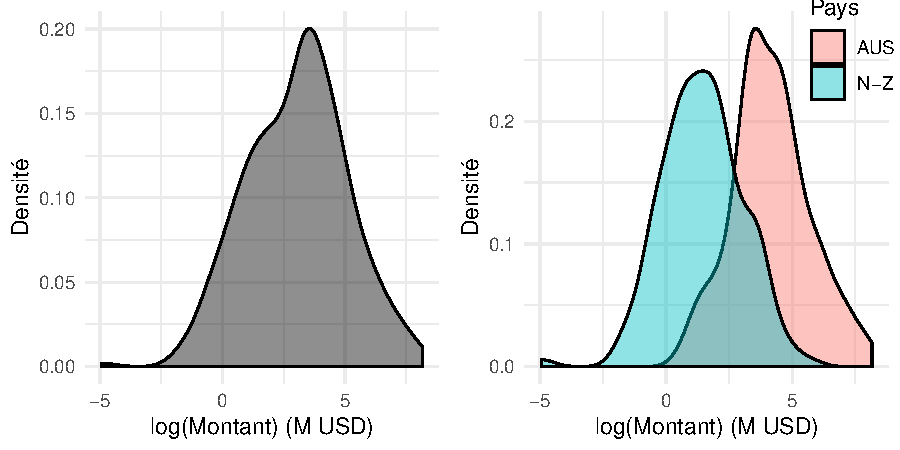
\includegraphics{images/fig-005}
\end{center}
\caption{Densité du logarithme du montant des catastrophes}
\label{fig:3.1}
\end{figure}

\begin{figure}[h]
\begin{center}
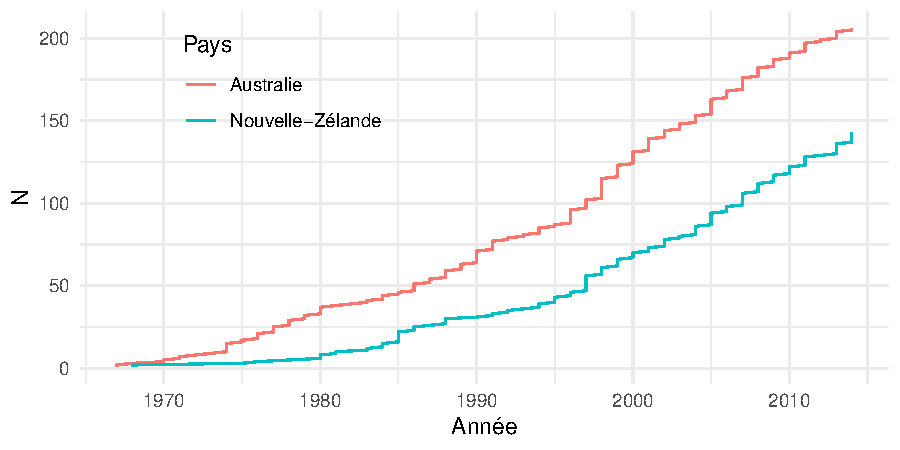
\includegraphics{images/fig-006}
\end{center}
\caption{Nombre cumulatif de catastrophes par pays}
\label{fig:3.2}
\end{figure}


\begin{figure}[h]
\begin{center}
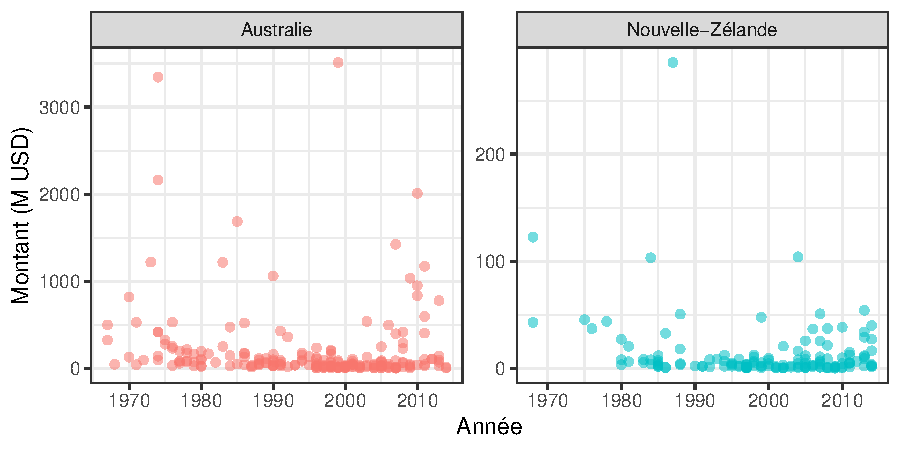
\includegraphics{images/fig-007}
\end{center}
\caption{Évolution des catastrophes par pays}
\label{fig:3.3}
\end{figure}   

% latex table generated in R 3.6.1 by xtable 1.8-4 package
% Mon Dec  2 15:08:47 2019
\begin{table}[ht]
\centering
\begin{tabular}{cccccccc}
  \hline
Type & N & Moyenne & Écart & Minimum & Médiane & Q3 & Maximum \\ 
  \hline
Bushfire & 26 & 143 & 259 & 7 & 39 & 134 & 1217 \\ 
  Cyclone & 37 & 325 & 675 & 2 & 88 & 217 & 3343 \\ 
  Earthquake & 9 & 56 & 91 & 0 & 25 & 47 & 286 \\ 
  Flood & 83 & 62 & 230 & 0 & 5 & 39 & 2010 \\ 
  Flood, Storm & 36 & 54 & 79 & 1 & 24 & 71 & 414 \\ 
  Hailstorm & 41 & 274 & 606 & 0 & 75 & 235 & 3511 \\ 
  Other & 12 & 121 & 296 & 2 & 6 & 50 & 1035 \\ 
  Power outage & 2 & 6 & 6 & 1 & 6 & 8 & 11 \\ 
  Storm & 86 & 97 & 228 & 0 & 28 & 57 & 1424 \\ 
  Tornado & 12 & 7 & 13 & 0 & 3 & 7 & 47 \\ 
  Weather & 4 & 11 & 11 & 2 & 6 & 13 & 27 \\ 
   \hline
\end{tabular}
\caption{Résumé statistique des montants (M USD) de catastrophes par Type} 
\label{tab:3.6}
\end{table}
\clearpage
\section{Approche classique}

Avant d'essayer la nouvelle méthode proposée, les méthodes classiques présentées à au chapitre \ref{chap:notions} sont appliquées pour être en mesure d'évaluer la valeur de la nouvelle méthode. Plus spécifiquement, l'approche \textit{POT} présentée à la section \ref{sec:pot} est appliquée dans la présente section étant donné que c'est ce type de modèle qui est appliqué dans les prochaines sections. À noter que les différents calculs de cette section nécessitant des techniques numériques sont faits avec le paquetage \texttt{ismev}. L'approche ici est donc de prendre l'ensemble des données, de choisir un seuil $u$ approprié et d'estimer les paramètres de la loi Pareto généralisée avec les excès de seuil, le tout en tenant compte d'aucunes variables exogènes. Comme mentionné, la première étape de cette méthodologie est le choix de la valeur du seuil $u$. La première méthode demande de tracer le \textit{mean residual plot} dont les points mentionnés dans l'équation \ref{eq:1.2.5}. Après un certaine valeur $u$ pour lequel la distribution est appropriée, le graphique devrait être linéaire en $u$. La figure \ref{fig:3.4} montre que déjà à partir de petites valeurs, cette conditon est respectée, il est ensuite difficile, voire subjectif de choisir une valeur précise. Ici, le graphique suggère de sélectionner une valeur entre 0 et 10.
\begin{figure}[h]
\begin{center}
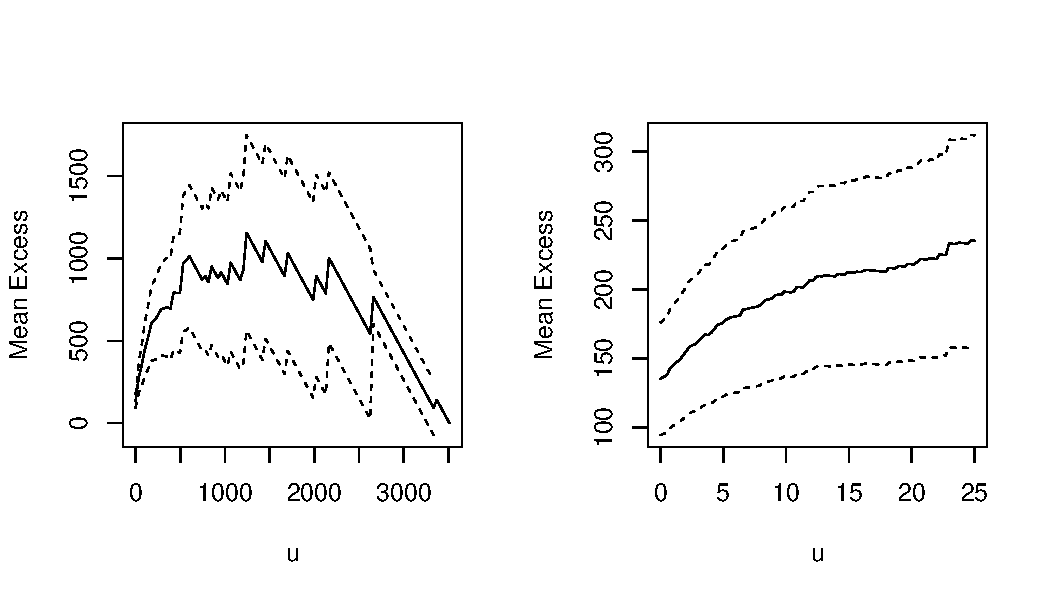
\includegraphics{images/fig-009}
\end{center}
\caption{\textit{Mean residual plot}}
\label{fig:3.4}
\end{figure}

La deuxième méthode mentionnée à la section \ref{sec:pot} propose d'estimer les paramètres du modèle pour différentes valeurs de $u$. Comme expliqué dans cette section, $\sigma^*$ et $\xi$ devraient rester constants au-delà de $u_0$. La figure \ref{fig:3.5} montre des résulats plus concluants que la figure \ref{fig:3.4}. En effet, les valeurs de $\sigma^*$ et de $\xi$ deviennent constantes environ à $u=10$. L'analyse des deux différentes techniques de sélection de seuil mènent donc à une sélection de $u=10$. Environ 64\% des données dépassent ce seuil, un bon nombre de données est donc utile pour la modélisation des excès.
\begin{figure}[h]
\begin{center}
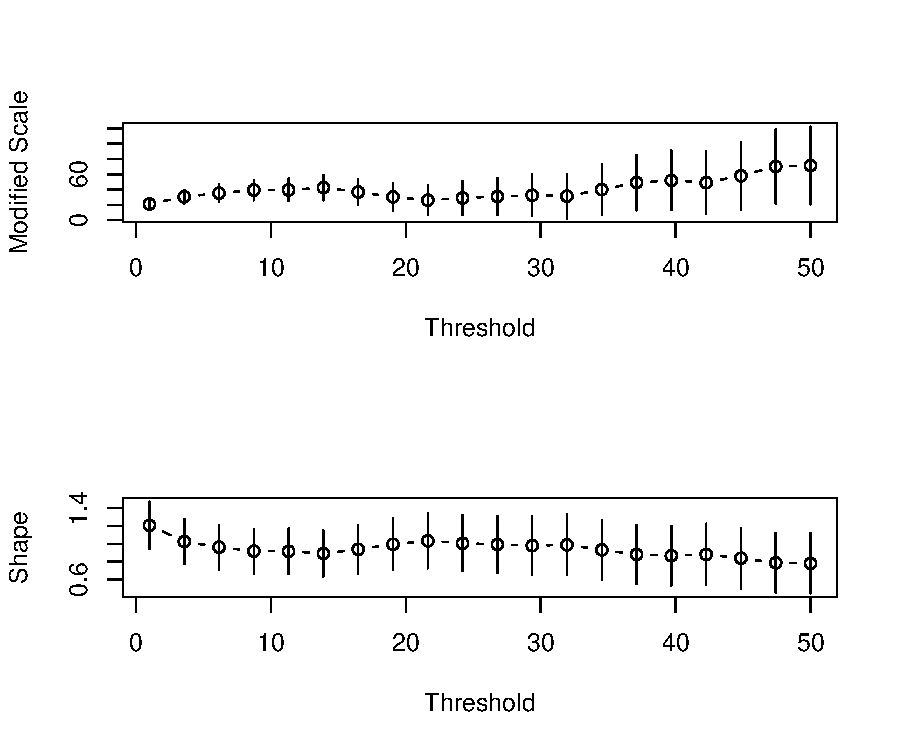
\includegraphics{images/fig-010}
\end{center}
\caption{Estimation des paramètres du modèle pour différents seuils}
\label{fig:3.5}
\end{figure}

Après avoir sélectionné le seuil, il faut ensuite estimer les paramètres de la loi Pareto généralisée avec la méthode du maximum de vraisemblance. Les différents détails de ce calcul se trouvent dans les équations \ref{eq:1.2.6} et \ref{eq:1.2.7}. Voici les résultats obtenus avec un intervalle de confiance de 95 \%.

\begin{equation*}
\begin{gathered}
(\hat\sigma,\hat\xi) = (49.329951;\ 0.941132)\\
\ell(\hat\sigma,\hat\xi) = -1308.013\\
\text{Var}(\hat\sigma) = 41.9446912\\
\text{Var}(\hat\xi) = 0.01673518
\end{gathered}
\end{equation*}
\

\begin{equation*}
\begin{gathered}
\hat\zeta_u = 0.6418338\\
\text{Var}(\hat\zeta_u) = 0.000658691
\end{gathered}
\end{equation*}
\

\begin{equation*}
\begin{gathered}
IC_{\hat\sigma} = (36.6362993;\ 62.023603)\\
IC_{\hat\xi} = (0.6875822;\ 1.194682)\\
IC_{\hat\zeta_u} = (0.5915314;\ 0.6921362)
\end{gathered}
\end{equation*}
\

Suite aux résultats obtenus, les graphiques de validation mentionnés à la section \ref{sec:pot} peuvent être tracés pour juger de la qualité du modèle. La figure \ref{fig:3.6} montre des résultats qui ne sont pas désastreux, mais qui sont loin d'être concluants en ce qui concerne l'ajustement des données au modèle proposé dans la présente section. Le graphique \textit{P-P} est tout de même adéquat, mais les trois autres graphiques sont loins de l'être. Les graphiques \textit{Q-Q} et celui de la densité obtenue montrent que le modèle représentent mal les données utilisées et le graphique des niveaux de retour montre que dès que la période de retour est un peu élevé, le niveau obtenu est extrêmement volatile. 
\


Pour conclure, le modèle proposé dans cette section représente un modèle de base qui considère toutes les données de la manière sans égard aux informations supplémentaires disponibles par rapport aux montants des catastrophes. Il n'est donc pas surprenant de voir que cette approche n'est pas tout à fait adéquate dans le cas présent, mais reste que cette approche est viable, rapide et peut être une bonne solution lorsque seulement les montants sont disponibles. Il est également important de savoir que le modèle testé dans cette section est la base de tous autres modèles plus avancés, tous comme les modèles qui seront testés aux prochaines sections.
\begin{figure}[h]
\begin{center}
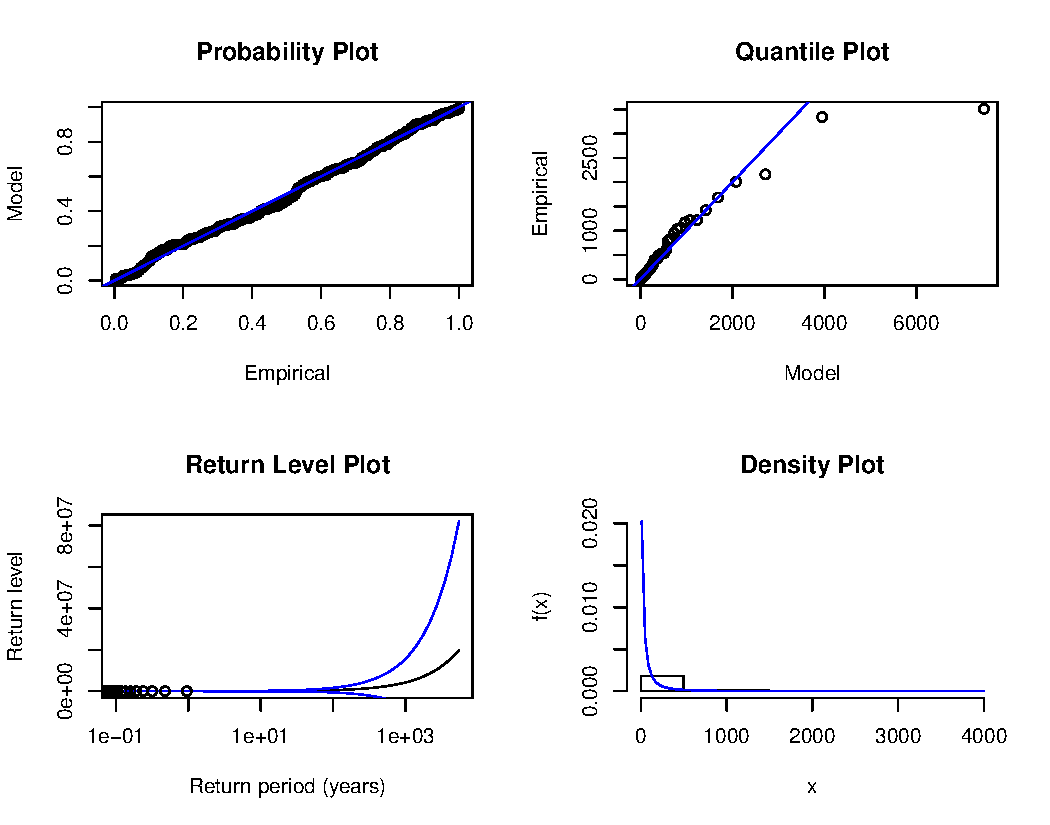
\includegraphics{images/fig-011}
\end{center}
\caption{Graphiques de validation du modèle}
\label{fig:3.6}
\end{figure}


\clearpage
\section{Approche dynamique à deux variables}
\label{sec:3.3}

Cette section applique la méthodologie et le modèle proposés au chapitre \ref{chap:article} avec deux variables, l'année et le pays. On considère donc une variable numérique de temps ainsi qu'une variable catégorique à deux niveaux. Seulement deux variables sont initialemment utilisées étant donné que c'est ce que l'article étudié utilise pour ilustrer la méthode. De plus, étant donné le nombre limité de données disponibles, il est préférable de ne pas commencer avec un nombre de sous-groupes trop élevés. Une troisième variable sera considérée à la section \ref{sec:3.4}. Avant même de commencer, les figures \ref{fig:3.1} et \ref{fig:3.2} suggèrent que les paramètres du modèles devraient bel et bien varier entre les deux pays et à travers le temps. Dans le cadre de la modélisation, seulement l'ajustement du paramètre $\rho$ est inclu dans le rapport, voir \ref{eq:2.2.13}. Un seuil de valeur 10 M USD est toujours utilisé, voir les figures \ref{fig:3.4} et \ref{fig:3.5}. 
\\

Premièrement, le paramètre $\rho$ du modèle est ajusté aux données. Après avoir statistiquement comparé les différents modèles, le modèle sélectionné pour $\hat\rho$ dépend du pays et du temps et a la forme suivante:
\begin{equation}\label{eq:3.3.1}
\log\Bigg(\frac{\hat\rho(x,t)}{1-\hat\rho(x,t)}\Bigg) = \hat{f}_\rho(pays) + \hat{h}^{(2)}_\rho(annee)
\end{equation}
où ${h}^{(\text{Df})}$ représente une spline naturelle quadratique avec $\text{Df}$ degrés de liberté.
\\


Voici une représentation graphique des résultats obtenus.
\begin{figure}[h]
\begin{center}
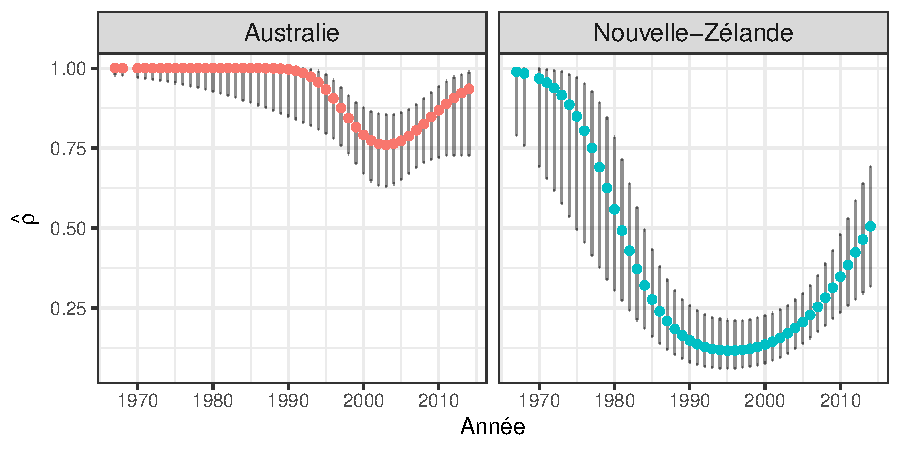
\includegraphics{images/fig-013}
\end{center}
\caption{Prédictions du taux d'excès de seuil avec intervalles de confiance à 95\%}
\label{fig:3.7}
\end{figure}

La figure \ref{fig:3.7} indique qu'il y a bel et bien une différence entre les pays et à travers le temps. Plus spécifiquement, les catastrophes australiennes dépassent beaucoup plus souvent le seuil de 10 millions et la figure indique également un paramètre élevé et constant pendant quelques années pour ensuite observé une diminution de celui-ci pour que finalement celui-ci remonte à un certain niveau.
\\

Ensuite, les paramètres de la loi Pareto généralisée sont ajustés aux données. Après avoir statistiquement comparé les différents modèles, le modèle sélectionné pour $\hat\xi$ dépend du pays et non du temps et a la forme suivante:
\begin{equation}\label{eq:3.3.2}
\hat\xi(x,t) = \hat{f}_\xi(pays)
\end{equation}

De son côté, le modèle sélectionné pour $\hat\beta$ dépend du pays et du temps et a la forme suivante:
\begin{equation}\label{eq:3.3.3}
\hat\beta(x,t) = \hat{f}_\beta(pays) + \hat{h}^{(3)}_\beta(annee)
\end{equation}



Les figures \ref{fig:3.8} et \ref{fig:3.9} présentent une représentation graphique des résultats obtenus pour les deux paramètres.
\begin{figure}[h]
\begin{center}
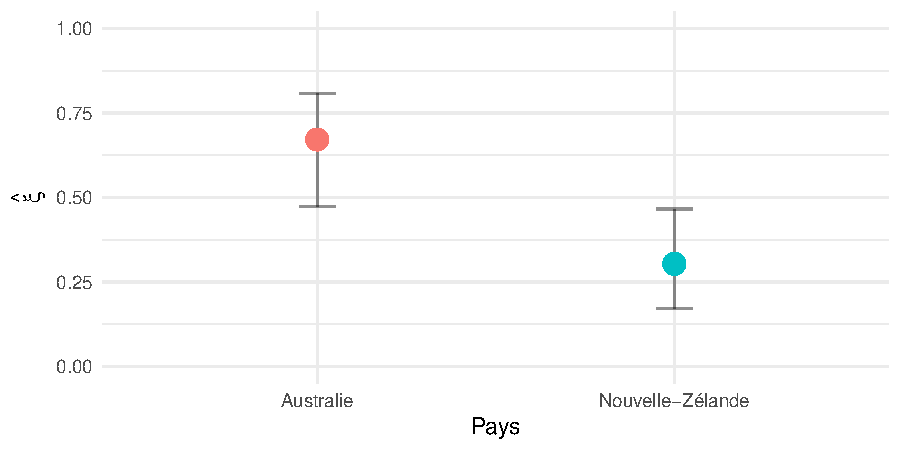
\includegraphics{images/fig-015}
\end{center}
\caption{Prédictions du paramètre $\xi$ avec intervalles de confiance à 95\%}
\label{fig:3.8}
\end{figure}

La figure \ref{fig:3.8} montre qu'il y a bel et bien une différence entre les deux pays et que cette différence est très importante. Le fait que le paramètre de l'Australie soit plus élevé fait du sens, car la distribution des catastrophes australiennes a une queue plus épaisse que celle des catastrophes de la Nouvelle-Zélande. 
\\

\begin{figure}[h]
\begin{center}
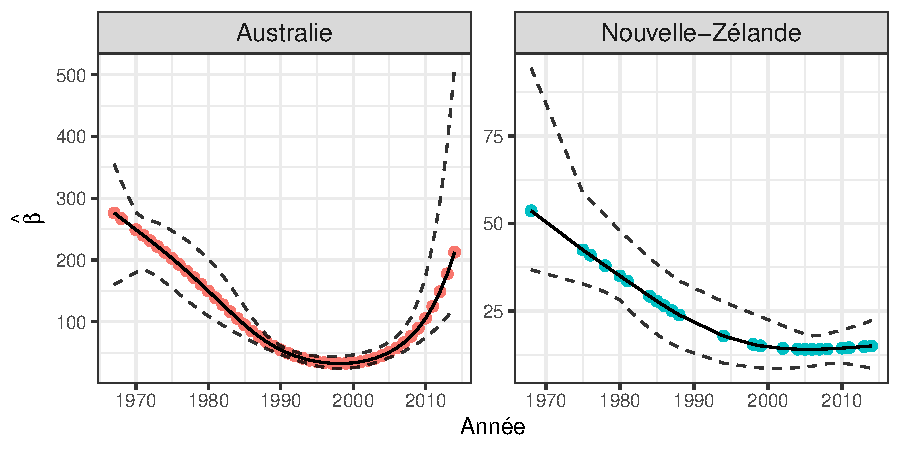
\includegraphics{images/fig-016}
\end{center}
\caption{Prédictions du paramètre $\beta$ avec intervalles de confiance à 95\%}
\label{fig:3.9}
\end{figure}

La figure \ref{fig:3.9} montre bien que les deux variables sélectionnées ont bel et bien un impact sur le paramètre $\beta$. Tout comme avec $\xi$, il est logique que les paramètres de la Nouvelle-Zélande soient inférieurs que ceux de l'Australie tout simplement parce que les pertes sont généralement plus élevées, voir la figure \ref{fig:3.1}. La figure montre également que, de façon générale, le paramètre dimiunue avec le temps.
\\

Même si les paramètres du modèle sont maintenant obtenus, il est important de vérifier l'adéquation du modèle avant d'effectuer n'importe quelle inférence. Comme l'explique l'équation \ref{eq:2.2.12}, une validation possible est de vérifier si les $r_i$ se comportent comme des variables aléatoires indépendantes suivant une loi exponentielle standards. Le graphique \textit{Q-Q} de cette loi est donc tracé à la figure \ref{fig:3.10}.

La figure montre que la calibration du modèle n'est pas tout si mal et même bonne dans l'ensemble. Le graphique n'est pas catastrophique et tout de même mieux que celui de la figure \ref{fig:3.6}. Peut-être que l'ajout d'une troisième variable à la section \ref{sec:3.4} va améliorer la qualité du modèle obtenu.
\\

Ensuite, à l'aide de l'équation \ref{eq:2.2.13}, les différentes $\widehat{\text{VaR}_{0.99}}$ peuvent être calculées. La figure \ref{fig:3.11} montre les résultats. 
\begin{figure}[h]
\begin{center}
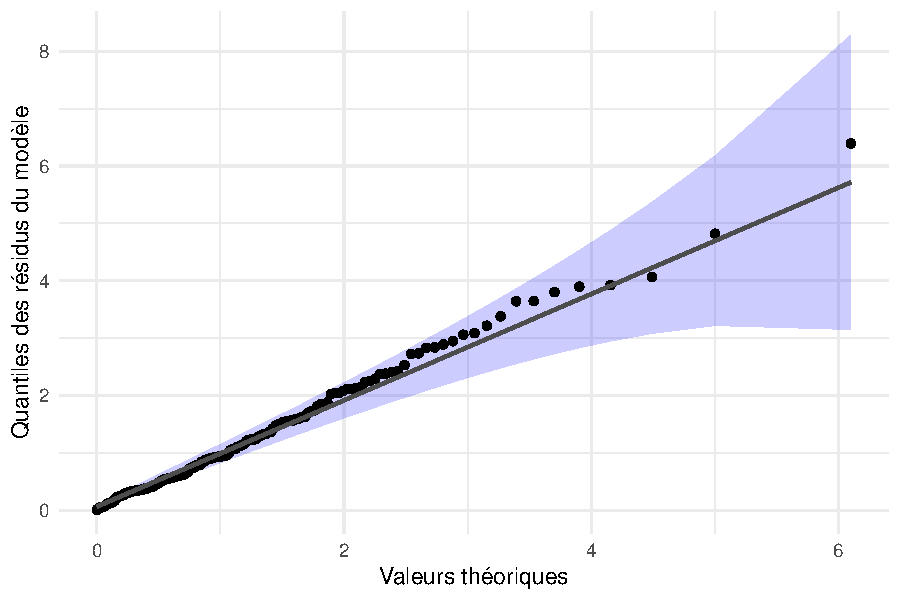
\includegraphics{images/fig-018}
\end{center}
\caption{Graphique \textit{Q-Q} de $\text{Exp}(1)$}
\label{fig:3.10}
\end{figure}

\begin{figure}[h]
\begin{center}
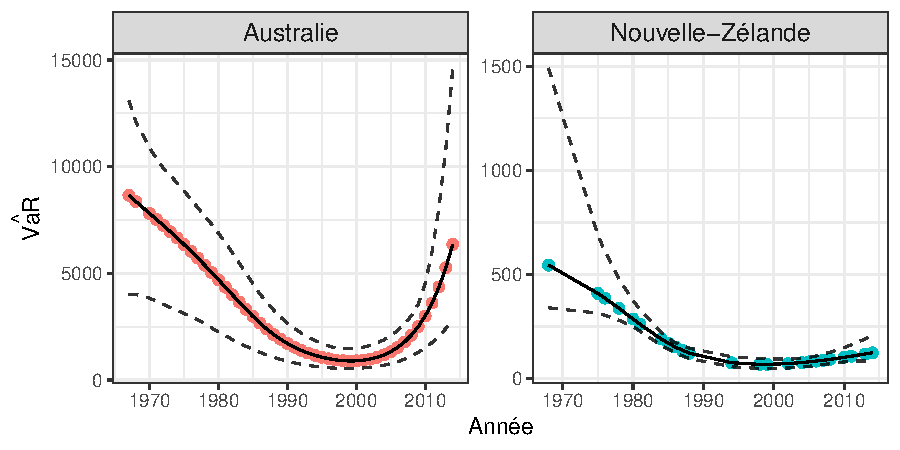
\includegraphics{images/fig-019}
\end{center}
\caption{$\widehat{\text{VaR}_{0.99}}$ avec intervalles de confiance à 95\%}
\label{fig:3.11}
\end{figure}

Il est logique de voir que la mesure de risque dépend du temps et du pays car celle-ci est obtenue avec les paramètres estimés. Tout comme avec les paramètres, il est logique que les valeurs obtenues pour la Nouvelle-Zélande soient inférieurs que celles de l'Australie tout simplement parce que les pertes sont généralement plus élevées pour l'Australie.
\\

C'est ce qui conclut cette section. La méthodologie proposée par les auteurs fonctionne et donnent les résultats escomptés lorque le temps ainsi qu'une variable catégorique sont considérés. Le modèle final obtenu n'est pas parfait, mais est tout de même une amélioration du modèle classique vu à la section \ref{sec:pot}.


\clearpage
\section{Approche dynamique à trois variables}
\label{sec:3.4}

Dans cette section, la même procédure que la section \ref{sec:3.3} est employée, mais la variable représentant le type de catastrophes est maintenant disponible. Un seuil de 10 M USD est toujours utilisé. Il y a 11 types différents dans les données. Une démarche complète de modélisation a été faite avec tous les types non regroupés, mais étant donné le nombre limité de données, les résultats ne furent pas concluants et les détails de ce modèle ne sont pas incluts dans ce rapport. Pour être en mesure de travailler avec cette troisième variable, un regroupement des types a dû être fait. La table \ref{tab:3.7} présente un résumé de ce regroupement. Sans même commencer la modélisation, la table \ref{tab:3.6} montre que le type de catastrophes va probablement s'avérer significatif pour les différents paramètres du modèle étant donnée que la distribution du montant de catastrophe varie beaucoup entre les différents types. 


% latex table generated in R 3.6.1 by xtable 1.8-4 package
% Mon Dec  2 15:11:12 2019
\begin{table}[ht]
\centering
\begin{tabular}{cc}
  \hline
Type & Type2 \\ 
  \hline
Bushfire & Bushfire \\ 
  Hailstorm & Hailstorm \\ 
  Cyclone & Cyclone \\ 
  Flood & Flood, Storm \\ 
  Flood, Storm & Flood, Storm \\ 
  Storm & Flood, Storm \\ 
  Other & Other \\ 
  Tornado & Other \\ 
  Earthquake & Other \\ 
  Weather & Other \\ 
  Power outage & Other \\ 
   \hline
\end{tabular}
\caption{Regroupement des types de catastrophes} 
\label{tab:3.7}
\end{table}
Tout comme lors de section précédente, le paramètre $\rho$ du modèle est le premier à être ajusté aux données. Après avoir statistiquement comparé les différents modèles, le modèle sélectionné pour $\hat\rho$ dépend du pays, du type et du temps et a la forme suivante:
\begin{equation}\label{eq:3.4.1}
\log\Bigg(\frac{\hat\rho(x,t)}{1-\hat\rho(x,t)}\Bigg) = \hat{f}_\rho(pays) + \hat{f}_\rho(type) + \hat{h}^{(2)}_\rho(annee)
\end{equation}

La figure \ref{fig:3.12} montre les résultats pour l'Australie et la figure ref{fig:3.13} montre ceux pour la Nouvelle-Zélande.
\\



\begin{figure}[h]
\begin{center}
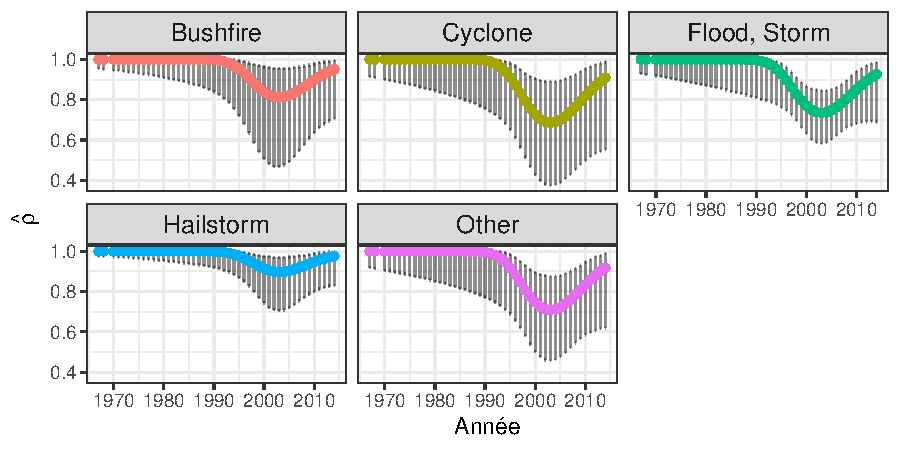
\includegraphics{images/fig-023}
\end{center}
\caption{Prédictions du paramètre $\rho$ pour l'Australie avec intervalles de confiance à 95\%}
\label{fig:3.12}
\end{figure}

\begin{figure}[h]
\begin{center}
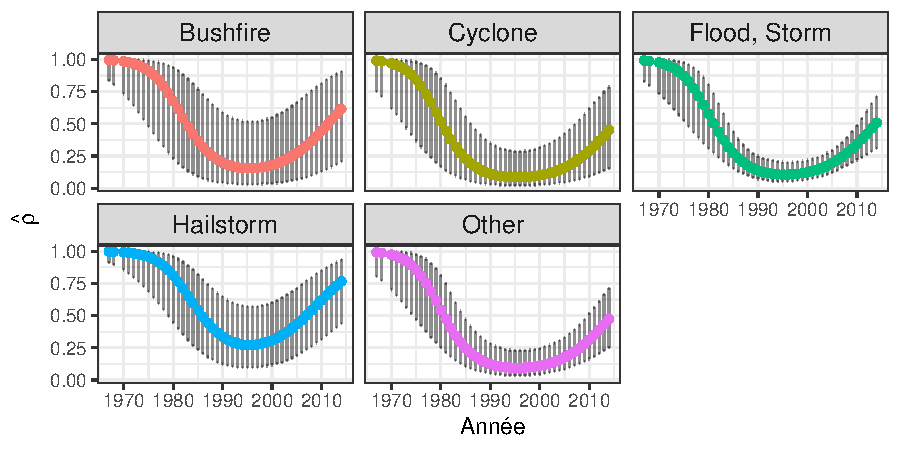
\includegraphics{images/fig-024}
\end{center}
\caption{Prédictions du paramètre $\rho$ pour la Nouvelle-Zélande avec intervalles de confiance à 95\%}
\label{fig:3.13}
\end{figure}

Les deux figures montrent que, comme dans la section précédente, il est clair que le paramètre est différent entre les deux pays et que celui-ci dépend du temps. De plus, même si cela est moins significatif que les pour les autres variables, les figures montrent également que le type de catastrophes est important pour la détermination du paramètre. Les courbes sont semblables par pays, mais le type amène une certaine translation verticale de la courbe. Cependant, on peut voir que les intervalles de confiance sont plus larges que ceux de la figure \ref{fig:3.7} étant donné qu'il y a maintenant moins de données par sous-groupes de variables.
\\

Suivant à nouveau la même démarche que la section précédente, les paramètres de la loi Pareto généralisée sont ajustés aux données. Après avoir statistiquement comparé les différents modèles, le modèle sélectionné pour $\hat\xi$ dépend du pays, du type et non du temps et a la forme suivante:
\begin{equation}\label{eq:3.4.2}
\hat\xi(x,t) = \hat{f}_\xi(pays) + \hat{f}_\xi(type)
\end{equation}

De son côté, le modèle sélectionné pour $\hat\beta$ dépend du pays, du type et du temps et a la forme suivante:
\begin{equation}\label{eq:3.4.3}
\hat\beta(x,t) = \hat{f}_\beta(pays) + \hat{f}_\xi(type) + \hat{h}^{(4)}_\beta(annee)
\end{equation}


Les figures \ref{fig:3.14}, \ref{fig:3.15} et \ref{fig:3.16} présentent une représentation graphique des résultats obtenus pour les deux paramètres.
\begin{figure}[h]
\begin{center}
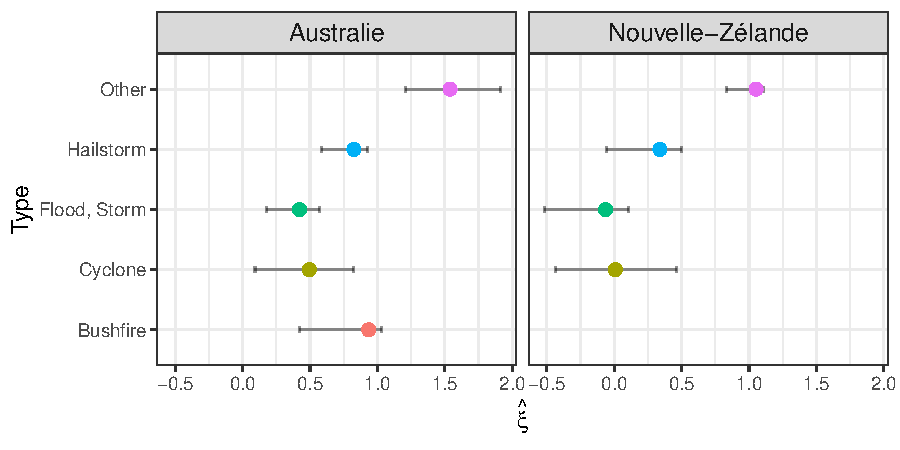
\includegraphics{images/fig-026}
\end{center}
\caption{Prédictions du paramètre $\xi$ avec intervalles de confiance à 95\%}
\label{fig:3.14}
\end{figure}

La figure \ref{fig:3.14} montre qu'il y a bel et bien une différence entre les différents types et que celle-ci est consirédablement importante. Ici, le comportement entre les types est semblable pour les deux pays, mais la figure montre clairement que les paramètres de l'Australie sont supérieurs à ceux de la Nouvelle-Zélande, ce qui est logique. De plus, contrairement aux résultats obtenus à la figure \ref{fig:3.8} où les résultats étaient non problématiques, les résultats obtenus ici contiennent deux valeurs (pour le même type) supérieures à 1, ce qui représente un modèle à moyenne infinie. Deux intervalles de confiance vont également jusqu'à des valeurs négatives sans toutefois atteindre -1, ce qui est très problématique.
\\

\begin{figure}[h]
\begin{center}
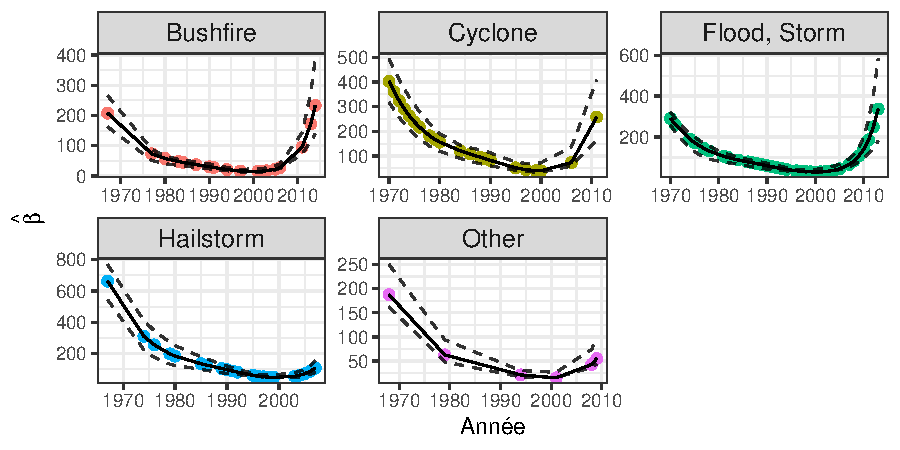
\includegraphics{images/fig-027}
\end{center}
\caption{Prédictions du paramètre $\beta$ pour l'Australie avec intervalles de confiance à 95\%}
\label{fig:3.15}
\end{figure}


\begin{figure}[h]
\begin{center}
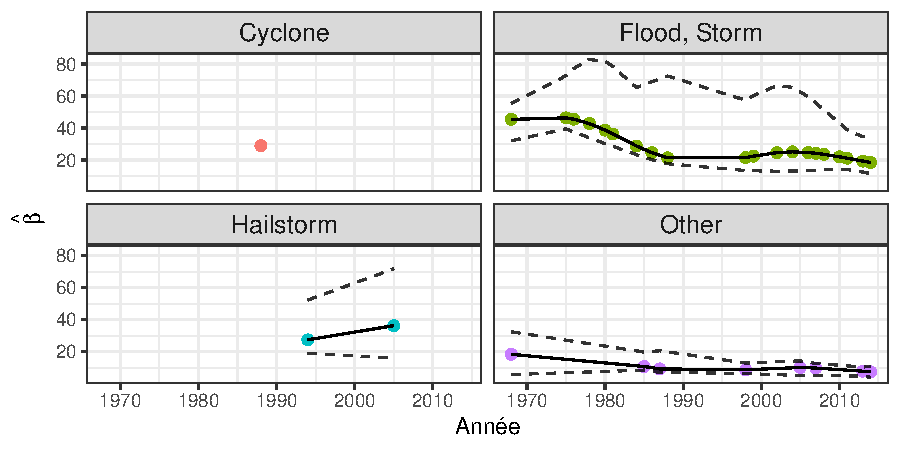
\includegraphics{images/fig-028}
\end{center}
\caption{Prédictions du paramètre $\beta$ pour la Nouvelle-Zélande avec intervalles de confiance à 95\%}
\label{fig:3.16}
\end{figure}

Les figures \ref{fig:3.15} et \ref{fig:3.16} montrent bien qu'encore une fois, le pays a une importance très significative pour la détermination des paramètres. De plus, même si cela est moins considérable que pour $\xi$, les figures montrent qu'il y a bel et bien une différence entre les différents types. Pour l'Australie, les courbes sont semblables, mais tout comme avec $\rho$, le type amène une certaine translation verticale de la courbe. Pour la Nouvelle-Zélande, le type amène également des courbes différentes. Un problème flagrant est remarquable à la figure \ref{fig:3.16} pour laquelle il y a très peu de points et donc des résultats peu crédibles. Ce problème est dû au fait qu'il y a déjà très peu de données et qu'en plus une troisième variable est rajoutée, ce qui rend les sous-groupes de covariables moins populés. Une autre cause vient du fait que seulement les données au-dessus du seuil $u$ sont utilisées pour la modélisation et la Nouvelle-Zélande présente beaucoup moins de pertes qui remplissent ce critère.
\\

Il est maintenant important de vérifier l'adéquation du modèle avant d'effectuer n'importe quelle inférence. Cette étape est également utile pour voir si l'ajout d'une troisième variable améliore le modèle. Le même type de graphique que la figure \ref{fig:3.10} est tracé à la figure \ref{fig:3.17}. 




\begin{figure}[h]
\begin{center}
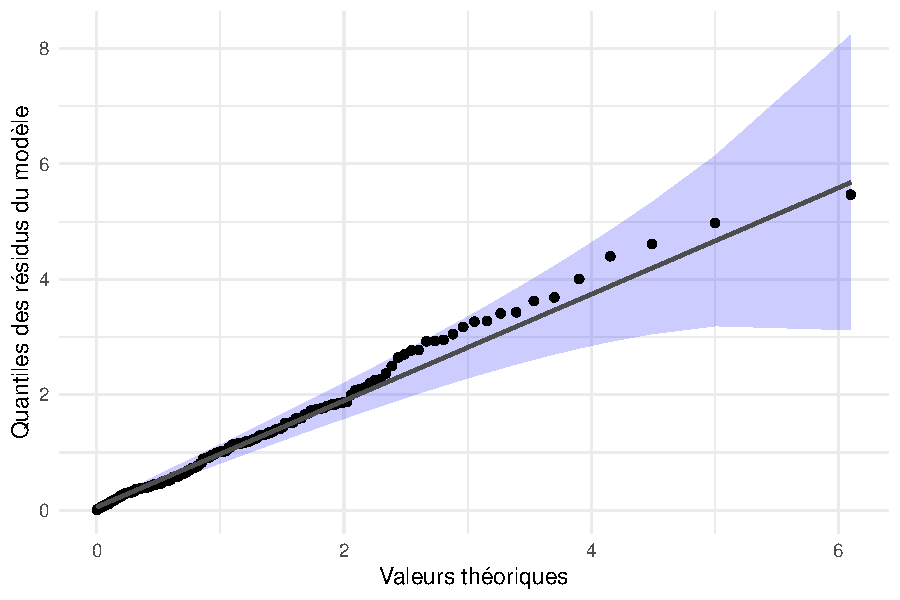
\includegraphics{images/fig-030}
\end{center}
\caption{Graphique \textit{Q-Q} de $\text{Exp}(1)$}
\label{fig:3.17}
\end{figure}

Le résultat obtenu à la figure \ref{fig:3.17} est, dans l'ensemble, très concluant, tout comme celui obtenu à la figure \ref{fig:3.10}. Il est difficile de dire lequel des graphiques est meilleur.


Les différentes $\widehat{\text{VaR}_{0.99}}$ peuvent maintenant être calculées. Les figures \ref{fig:3.18} et \ref{fig:3.19} montrent les résultats obtenus pour les deux pays. 
\begin{figure}[h]
\begin{center}
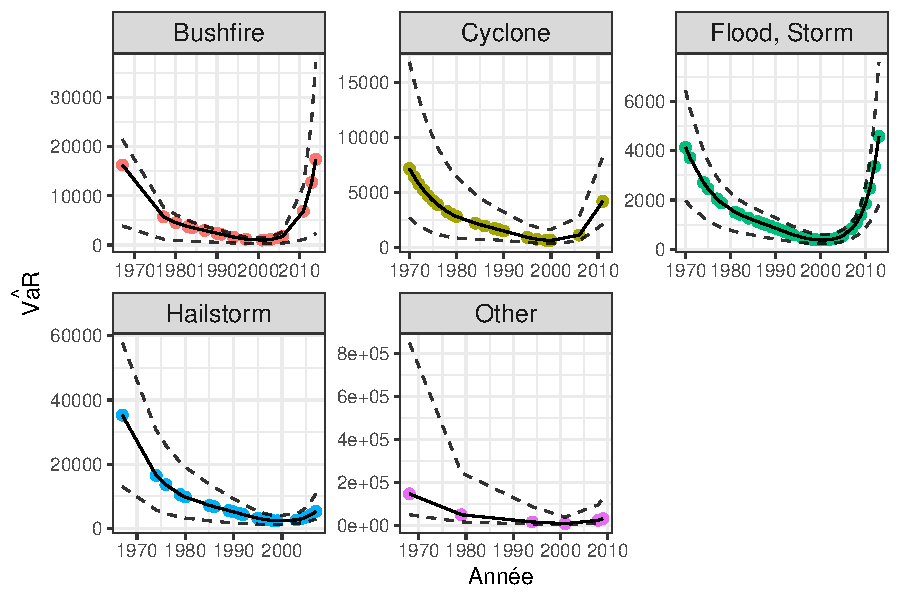
\includegraphics{images/fig-031}
\end{center}
\caption{$\widehat{\text{VaR}_{0.99}}$ avec intervalles de confiance à 95\%}
\label{fig:3.18}
\end{figure}

\begin{figure}[h]
\begin{center}
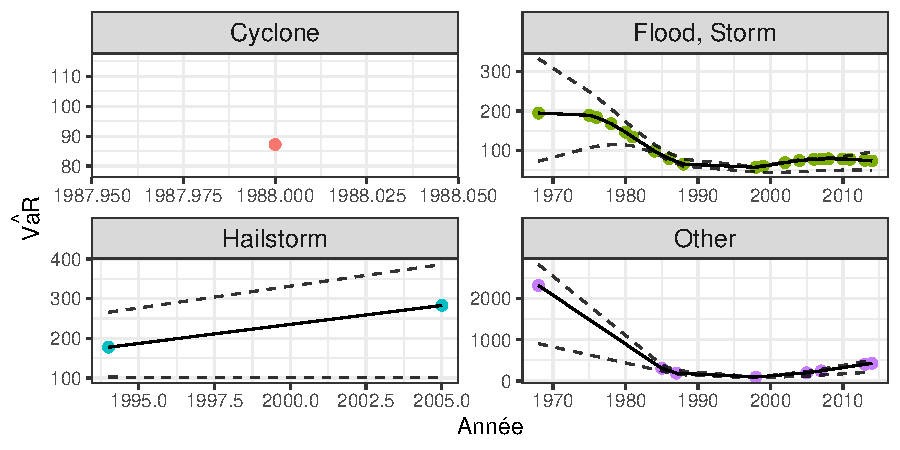
\includegraphics{images/fig-032}
\end{center}
\caption{$\widehat{\text{VaR}_{0.99}}$ avec intervalles de confiance à 95\%}
\label{fig:3.19}
\end{figure}

Tout comme à la section précédente, il est logique de voir que la mesure de risque dépend du temps, du type et du pays car celle-ci est obtenue avec les paramètres estimés et que les valeurs obtenues pour la Nouvelle-Zélande soient inférieurs que celles de l'Australie tout simplement parce que les pertes sont généralement plus élevées pour l'Australie.
\\

C'est ce qui conclut cette section. Cette section a montré que l'ajout d'une troisième variable catégorique est possible si celle-ci n'a pas trop de niveaux. Le modèle obtenu est adéquat, mais la qualité de celui-ci n'est pas grandement différente avec celle du modèle développé à la section \ref{sec:3.3} en plus que le modèle de la présente section présente des paramètres et des mesures de risques plus volatiles et moins crédibles. 


% Conclusion


\chapter*{Conclusion}
\label{chap:conclusion} 
\phantomsection\addcontentsline{toc}{chapter}{\nameref{chap:conclusion}}

\bibliography{biblio}


%\appendix

%%% Annexe
% le Sweaveopt



\chapter{Code \textsf{R}}
\label{chap:code} 



\definecolor{mygreen}{rgb}{0,0.6,0}
\definecolor{mygray}{rgb}{0.5,0.5,0.5}
\definecolor{mymauve}{rgb}{0.58,0,0.82}

\NoAutoSpacing

\lstset{ 
  backgroundcolor=\color{white},   % choose the background color; you must add \usepackage{color} or \usepackage{xcolor}; should come as last argument
  basicstyle=\footnotesize,        % the size of the fonts that are used for the code
  breakatwhitespace=false,         % sets if automatic breaks should only happen at whitespace
  breaklines=true,                 % sets automatic line breaking
  captionpos=b,                    % sets the caption-position to bottom
  commentstyle=\color{mymauve},    % comment style
  deletekeywords={...},            % if you want to delete keywords from the given language
  escapeinside={\%*}{*)},          % if you want to add LaTeX within your code
  extendedchars=true,              % lets you use non-ASCII characters; for 8-bits encodings only, does not work with UTF-8
  firstnumber=1,                % start line enumeration with line 1000
  frame=single,	                   % adds a frame around the code
  keepspaces=true,                 % keeps spaces in text, useful for keeping indentation of code (possibly needs columns=flexible)
  keywordstyle=\color{blue},       % keyword style
  language=R,                 % the language of the code
  morekeywords={*,...},            % if you want to add more keywords to the set
  numbers=none,                    % where to put the line-numbers; possible values are (none, left, right) 
  numbersep=5pt,                   % how far the line-numbers are from the code
  numberstyle=\tiny\color{mygray}, % the style that is used for the line-numbers
  rulecolor=\color{black},         % if not set, the frame-color may be changed on line-breaks within not-black text (e.g. comments (green here))
  showspaces=false,                % show spaces everywhere adding particular underscores; it overrides 'showstringspaces'
  showstringspaces=false,          % underline spaces within strings only
  showtabs=false,                  % show tabs within strings adding particular underscores
  stepnumber=2,                    % the step between two line-numbers. If it's 1, each line will be numbered
  stringstyle=\color{mygreen},     % string literal style
  tabsize=2,	                   % sets default tabsize to 2 spaces
  title=\lstname                   % show the filename of files included with \lstinputlisting; also try caption instead of title
}




Cette section contient l'ensemble du code \textsf{R} qui a été utilisé pour ce rapport. À noter que ceci n'est qu'une petite partie de l'ensemble de la programmation qui a été nécessaire pour le projet et que seulement le nécessaire est inclus. Par exemple, lorsque plusieurs modèles sont comparés, la démarche de sélection n'est pas inclue et seulement le modèle final est danc cet annexe.

\begin{lstlisting}
libs <- c('dplyr', 'ggplot2', 'gridExtra', 'ismev', 'evir', 'xtable',
          'summarytools', 'utils', 'QRM', 'CASdatasets', 'tidyr')
sapply(libs, require, character.only = T)

data("auscathist")
data("nzcathist")


print(
  xtable(descr(auscathist, stats = "common", transpose = T), caption = "Résumé statistique des variables numériques pour l'Australie", label="tab:3.1", align=rep("c",8), digits=0, table.placement="h")
)

print(
xtable(freq(auscathist$Type), caption = "Distribution du Type de catastrophe pour l'Australie", label="tab:3.2", align=rep("c",6), digits=0, table.placement="h")
)


print(
  xtable(descr(nzcathist, stats = "common", transpose = T), caption = "Résumé statistique des variables numériques pour la Nouvelle-Zélande", label="tab:3.3", align=rep("c",8), digits=3, table.placement="h")
)

print(
xtable(freq(nzcathist$Type), caption = "Distribution du Type de catastrophe pour la Nouvelle-Zélande", label="tab:3.4", align=rep("c",6), digits=0, table.placement="h")
)

tab <- data.frame(c(105.9, 974.7), c(114.8, 1039.0), c(0.7031, 0.6722))
rownames(tab) <- c("AUS", "NZ")
colnames(tab) <- c("IPC 2014", "IPC 2019", "Taux de change 2019")

print(
  xtable(tab, caption="Valeurs utilisées pour CostUS2019", label="tab:3.5", align=rep("c",4), digits=4, table.placement="h")
)

auscathist <- auscathist %>%
    select(Year, Quarter, FirstDay, Event, Type, Location, NormCost2014) %>%
    mutate(Country = as.factor("AUS"))

nzcathist <- nzcathist %>%
    select(Year, Quarter, FirstDay, Event, Type, Location, NormCost2014) %>%
    mutate(Country = as.factor("N-Z"))

auscathist <- auscathist %>%
    mutate(CostUS2019 = NormCost2014 * (114.8/105.9) * .7032) %>%
    select(-NormCost2014)

nzcathist <- nzcathist %>%
    mutate(CostUS2019 = NormCost2014 * (1039.0/974.7) * .6727) %>%
    select(-NormCost2014)

pacicathist <- rbind(auscathist, nzcathist) %>%
    dplyr::filter(CostUS2019 > 0) %>%
    mutate(Type = as.factor(Type)) %>%
    select(Year, Type, Country, CostUS2019)

colnames(pacicathist) <- c("Année", "Type", "Pays", "Montant")

pacicathist <- pacicathist %>% 
    dplyr::filter(Montant < 4000) %>% 
    dplyr::filter(Type != "Earthquake" | Montant < 2000)


grid.arrange(
  pacicathist %>%
    ggplot(aes(log(Montant))) +
    geom_density(alpha=.44, fill=1) +
    theme_minimal() +
    labs(x="log(Montant) (M USD)", y="Densité"),

  pacicathist %>% 
    ggplot(aes(log(Montant), fill=Pays)) + 
    geom_density(alpha=.44) + 
    theme_minimal() +
    labs(x="log(Montant) (M USD)", y="Densité") + 
    theme(legend.position = c(.9,.9)),
  
  ncol=2
)
  

levels(pacicathist$Pays)[levels(pacicathist$Pays)=="AUS"] <- "Australie"
levels(pacicathist$Pays)[levels(pacicathist$Pays)=="N-Z"] <- "Nouvelle-Zélande"

pacicathist %>% 
    group_by(Pays) %>%
    arrange(Année) %>% 
    mutate(cun = cumsum(as.numeric(Montant>0))) %>% 
    ungroup() %>% 
    ggplot(aes(x=Année, y=cun, col=Pays)) + 
    geom_line() +
    theme_minimal() +
    labs(y="N") + 
    theme(legend.position = c(.25,.8))
    
    
pacicathist %>% 
    ggplot() +
    geom_point(aes(x=Année, y=Montant, col=Pays)) + 
    facet_wrap(~Pays, scales="free") + 
    theme_bw() +
    theme(legend.position = "")+
    labs(y="Montant (M USD)")
    

print(
  xtable(data.frame(pacicathist %>% 
    group_by(Type) %>% 
    summarise(N = n(),
              Moyenne = mean(Montant),
              Écart = sd(Montant), 
              Minimum = min(Montant),
              Médiane = median(Montant),
              Q3 = quantile(Montant, .75),
              Maximum = max(Montant))), 
    caption = "Résumé statistique des montants (M USD) de catastrophes par Type", label="tab:3.6", align=rep("c",9), digits=0, table.placement="t"), include.rownames = FALSE)    


par(mfrow=c(1,2))
mrl.plot(pacicathist$Montant)
mrl.plot(pacicathist$Montant, umax = 25)


par(mfrow=c(1,1))
gpd.fitrange(pacicathist$Montant, 
             nint=20,
             umin=1, 
             umax = 50)
             
             
gpd.diag(gpd.fit(pacicathist$Montant, 10, show=FALSE))


paci.1 <- pacicathist %>% 
    select(-Type)

rate.exc.1 <- as.data.frame(paci.1 %>% 
                                mutate(rate.exc = as.numeric(Montant > 10)))


modrho <- gam(rate.exc ~ Pays + s(Année, fx=TRUE, k=2+1, bs="cr", by=Pays) - 1, 
              data=rate.exc.1, family=binomial(link=logit)) 


rhoFit <- QRM:::get.gam.fit(modrho)   

rhoPred <- QRM:::gam.predict(modrho, alpha=.05, value="rho")


rhoPred$predict <- exp(rhoPred$predict) / (exp(rhoPred$predict) + 1)
rhoPred$CI.low <- exp(rhoPred$CI.low) / (exp(rhoPred$CI.low) + 1)
rhoPred$CI.up <- exp(rhoPred$CI.up) / (exp(rhoPred$CI.up) + 1)



results.rho <- data.frame(rhoPred$covar, Pred=rhoPred$predict,
                          CI.low=rhoPred$CI.low, CI.up=rhoPred$CI.up)
                          

results.rho %>% 
    ggplot() + 
    geom_errorbar(aes(x=Année, ymin=CI.low, ymax=CI.up), alpha=.44, width=.1) +
    geom_point(aes(x=Année, y=Pred, col=Pays)) + 
    facet_wrap(~Pays) + 
    theme_bw() + 
    theme(legend.position = "", strip.text = element_text(size=12)) + 
    labs(y=expression(hat(rho)))
    

bootGPD <- QRM::gamGPDboot(paci.1, B=10, threshold=10, datvar="Montant",
                         
                         xiFrhs = ~ Pays - 1, 
                         nuFrhs = ~ Pays + s(Année, fx=TRUE, k=3+1, bs="cr", by=Pays) - 1, 
                         
                         niter=10, eps.xi=.005, eps.nu=.005)



xibetaFit <- QRM::get.GPD.fit(bootGPD, alpha=.05) 

xibetaPred <- QRM::GPD.predict(bootGPD)


results.xi <- data.frame(xibetaFit$xi$covar, Pred=xibetaFit$xi$fit,
                          CI.low=xibetaFit$xi$CI.low, CI.up=xibetaFit$xi$CI.up)


results.beta <- data.frame(xibetaFit$beta$covar, Pred=xibetaFit$beta$fit,
                         CI.low=xibetaFit$beta$CI.low, CI.up=xibetaFit$beta$CI.up)


results.xi %>% 
    ggplot() + 
    geom_errorbar(aes(x=Pays, ymin=CI.low, ymax=CI.up), alpha=.44, width=.1) +
    geom_point(aes(x=Pays, y=Pred, size=2, col=Pays)) + 
    theme_minimal() + 
    theme(legend.position = "", strip.text = element_text(size=12))+ 
    labs(y=expression(hat(xi))) +
    ylim(c(0,1))
    

results.beta %>% 
    ggplot() + 
    geom_point(aes(x=Année, y=Pred, col=Pays), size=2) + 
    geom_line(aes(x=Année, y=Pred)) + 
    geom_line(aes(x=Année, y=CI.low), linetype="dashed", alpha=.8) + 
    geom_line(aes(x=Année, y=CI.up), linetype="dashed", alpha=.8) + 
    facet_wrap(~Pays, scales="free") + 
    theme_bw() + 
    theme(legend.position = "", strip.text = element_text(size=12))+ 
    labs(y=expression(hat(beta)))
    
    
covar <- xibetaFit$beta$covar 


count.cov <- as.data.frame(covar %>% count(Pays))

vec.cov <- c()
for (i in nrow(count.cov):1){
    vec.cov <- c(rep(i, count.cov$n[i]), vec.cov)
}


xibetaFit$xi$fit <- xibetaFit$xi$fit[vec.cov]
xibetaFit$xi$CI.low <- xibetaFit$xi$CI.low[vec.cov]
xibetaFit$xi$CI.up <- xibetaFit$xi$CI.up[vec.cov]

xibetaFit$xi$covar <- covar



xibetaFit.xi.boot2 <- matrix(ncol = 10)
for (i in nrow(count.cov):1){
    xibetaFit.xi.boot2 <- rbind(
        do.call(rbind, replicate(count.cov$n[i], xibetaFit$xi$boot[i,], simplify=FALSE)),
        xibetaFit.xi.boot2
    )
}

xibetaFit$xi$boot <- xibetaFit.xi.boot2[-length(xibetaFit.xi.boot2[, 1]),]



xiFit.mat <- cbind(xibetaFit$xi$fit, xibetaFit$xi$boot)

betaFit.mat <- cbind(xibetaFit$beta$fit, xibetaFit$beta$boot)


rho.res <- data.frame(rhoFit$covar, rhoFit$fit)

rho.res.sel <- covar %>% 
    inner_join(rho.res)



final.results <- data.frame(Covar=xibetaFit$beta$covar,
                            rho = rho.res.sel$rhoFit.fit,
                            xi = xibetaFit$xi$fit,
                            xi.low = xibetaFit$xi$CI.low,
                            xi.up = xibetaFit$xi$CI.up,
                            beta = xibetaFit$beta$fit,
                            beta.low = xibetaFit$beta$CI.low,
                            beta.up = xibetaFit$beta$CI.up)





VaR <- cbind(covar, fit=sapply(1:(10+1), function(j)
    risk.measure(cbind(rho.res.sel$rhoFit.fit, xiFit.mat[,j], betaFit.mat[,j]),
                 alpha=.99, u=10, method="VaR")
))

VaR.boot <- VaR %>% select(-Pays, -Année, -fit.1)

VaR.fit <- data.frame(covar, 
                      fit    = VaR[, "fit.1"], 
                      CI.low = apply(VaR.boot, 1, quantile, probs=.05/2),
                      CI.up  = apply(VaR.boot, 1, quantile, probs=1-.05/2))



final.results <- final.results %>% 
    rename(Pays = Covar.Pays,
           Année = Covar.Année) 


paci.1.param <- paci.1 %>% 
    inner_join(final.results) %>% 
    
    dplyr::filter(Montant > 10) %>% 
    mutate(Y = Montant - 10)



paci.1.param$ri <- sapply(1:nrow(paci.1.param), 
                          function(i) -log(1 - pGPD(paci.1.param$Y[i], 
                                                    paci.1.param$xi[i], 
                                                    paci.1.param$beta[i])))


require(qqplotr)
paci.1.param %>% 
    ggplot(aes(sample = ri)) +
    stat_qq_band(distribution = "exp", dparams = 1, conf = .95, alpha=.2, fill="blue") +
    stat_qq_point(distribution = "exp", dparams = 1) + 
    stat_qq_line(distribution = "exp", dparams = 1,) + 
    theme_minimal() +
    labs(x="Valeurs théoriques", y="Quantiles des résidus du modèle")
    
    
VaR.fit %>%  
    ggplot() + 
    geom_point(aes(x=Année, y=fit, col=Pays), size=2) + 
    geom_line(aes(x=Année, y=fit)) + 
    geom_line(aes(x=Année, y=CI.low), linetype="dashed", alpha=.8) + 
    geom_line(aes(x=Année, y=CI.up), linetype="dashed", alpha=.8) + 
    facet_wrap(~Pays, scales = "free") + 
    theme_bw() + 
    theme(legend.position = "", strip.text = element_text(size=12)) +
    labs(y=expression(hat(VaR)))
    
    
paci.3 <- pacicathist

Type2 <- data.frame(Type = c("Bushfire", "Hailstorm", "Cyclone", 
                             "Flood", "Flood, Storm", "Storm", 
                             "Other", "Tornado", "Earthquake", "Weather", "Power outage"),
                    Type2 = c("Bushfire", "Hailstorm", "Cyclone",
                              rep("Flood, Storm",3), 
                              rep("Other",5)))

paci.3 <- paci.3 %>% 
    inner_join(Type2)

paci.3 %>% 
    count(Type2) %>% 
    arrange(-n)


paci.3 <- paci.3 %>% 
    mutate(Type=as.factor(Type2)) %>% 
    select(-Type2)


paci.3 <- droplevels(paci.3)


print(
  xtable(Type2, caption = "Regroupement des types de catastrophes", label="tab:3.7", align=rep("c",3), digits=0, table.placement="h"), include.rownames = FALSE
)


rate.exc.3 <- as.data.frame(paci.3 %>% 
                                mutate(rate.exc = as.numeric(Montant > 10)))

modrho <- gam(rate.exc ~ Pays + s(Année, fx=TRUE, k=2+1, bs="cr", by=Pays) + Type - 1, 
              data=rate.exc.3, family=binomial(link=logit))


rhoFit <- QRM:::get.gam.fit(modrho)   

rhoPred <- QRM:::gam.predict(modrho, alpha=.05, value="rho")


rhoPred$predict <- exp(rhoPred$predict) / (exp(rhoPred$predict) + 1)
rhoPred$CI.low <- exp(rhoPred$CI.low) / (exp(rhoPred$CI.low) + 1)
rhoPred$CI.up <- exp(rhoPred$CI.up) / (exp(rhoPred$CI.up) + 1)


results.rho <- data.frame(rhoPred$covar, Pred=rhoPred$predict,
                          CI.low=rhoPred$CI.low, CI.up=rhoPred$CI.up)


results.rho %>% 
    dplyr::filter(Pays == "Australie") %>% 
    ggplot() + 
    geom_errorbar(aes(x=Année, ymin=CI.low, ymax=CI.up), alpha=.44, width=.1) +
    geom_point(aes(x=Année, y=Pred, col=Type)) + 
    facet_wrap(~Type) + 
    theme_bw() + 
    theme(legend.position = "", strip.text = element_text(size=12)) + 
    labs(y=expression(hat(rho)))


results.rho %>% 
    dplyr::filter(Pays == "Nouvelle-Zélande") %>% 
    ggplot() + 
    geom_errorbar(aes(x=Année, ymin=CI.low, ymax=CI.up), alpha=.44, width=.1) +
    geom_point(aes(x=Année, y=Pred, col=Type)) + 
    facet_wrap(~Type) + 
    theme_bw() + 
    theme(legend.position = "", strip.text = element_text(size=12)) + 
    labs(y=expression(hat(rho)))
    

bootGPD <- QRM::gamGPDboot(paci.3, B=10, threshold=10, datvar="Montant",
                            
                            xiFrhs = ~ Pays + Type - 1,  
                            nuFrhs = ~ Pays + Type + s(Année, fx=TRUE, k=4+1, bs="cr", by=Pays) - 1, 
                            
                            niter=10, eps.xi=.005, eps.nu=.005)





xibetaFit <- QRM::get.GPD.fit(bootGPD, alpha=.05) 

xibetaPred <- QRM::GPD.predict(bootGPD)



results.xi <- data.frame(xibetaFit$xi$covar, Pred=xibetaFit$xi$fit,
                         CI.low=xibetaFit$xi$CI.low, CI.up=xibetaFit$xi$CI.up)


results.beta <- data.frame(xibetaFit$beta$covar, Pred=xibetaFit$beta$fit,
                           CI.low=xibetaFit$beta$CI.low, CI.up=xibetaFit$beta$CI.up)


results.xi %>% 
    ggplot() + 
    geom_errorbar(aes(x=Type, ymin=CI.low, ymax=CI.up), alpha=.44, width=.1) +
    geom_point(aes(x=Type, y=Pred, col=Type), size=2.5) + 
    coord_flip() + 
    facet_wrap(~Pays) + 
    theme_bw() + 
    theme(legend.position = "", strip.text = element_text(size=12)) + 
    labs(y=expression(hat(xi)))


results.beta %>% 
    dplyr::filter(Pays=="Australie") %>% 
    ggplot() + 
    geom_point(aes(x=Année, y=Pred, col=Type), size=2) + 
    geom_line(aes(x=Année, y=Pred)) + 
    geom_line(aes(x=Année, y=CI.low), linetype="dashed", alpha=.8) + 
    geom_line(aes(x=Année, y=CI.up), linetype="dashed", alpha=.8) + 
    facet_wrap(~Type, scales = "free") + 
    theme_bw() + 
    theme(legend.position = "", strip.text = element_text(size=12)) + 
    labs(y=expression(hat(beta)))
    

results.beta %>% 
    dplyr::filter(Pays=="Nouvelle-Zélande") %>% 
    ggplot() + 
    geom_point(aes(x=Année, y=Pred, col=Type), size=2) + 
    geom_line(aes(x=Année, y=Pred)) + 
    geom_line(aes(x=Année, y=CI.low), linetype="dashed", alpha=.8) + 
    geom_line(aes(x=Année, y=CI.up), linetype="dashed", alpha=.8) + 
    facet_wrap(~Type, ) + 
    theme_bw() + 
    theme(legend.position = "", strip.text = element_text(size=12)) + 
    labs(y=expression(hat(beta)))
    
    
covar <- xibetaFit$beta$covar 


count.cov <- as.data.frame(covar %>% count(Pays, Type))

vec.cov <- c()
for (i in nrow(count.cov):1){
    vec.cov <- c(rep(i, count.cov$n[i]), vec.cov)
}


xibetaFit$xi$fit <- xibetaFit$xi$fit[vec.cov]
xibetaFit$xi$CI.low <- xibetaFit$xi$CI.low[vec.cov]
xibetaFit$xi$CI.up <- xibetaFit$xi$CI.up[vec.cov]

xibetaFit$xi$covar <- covar



xibetaFit.xi.boot2 <- matrix(ncol = 10)
for (i in nrow(count.cov):1){
    xibetaFit.xi.boot2 <- rbind(
        do.call(rbind, replicate(count.cov$n[i], xibetaFit$xi$boot[i,], simplify=FALSE)),
        xibetaFit.xi.boot2
    )
}

xibetaFit$xi$boot <- xibetaFit.xi.boot2[-length(xibetaFit.xi.boot2[, 1]),]



xiFit.mat <- cbind(xibetaFit$xi$fit, xibetaFit$xi$boot)

betaFit.mat <- cbind(xibetaFit$beta$fit, xibetaFit$beta$boot)


rho.res <- data.frame(rhoFit$covar, rhoFit$fit)

rho.res.sel <- covar %>% 
    inner_join(rho.res)



final.results <- data.frame(Covar=xibetaFit$beta$covar,
                            rho = rho.res.sel$rhoFit.fit,
                            xi = xibetaFit$xi$fit,
                            xi.low = xibetaFit$xi$CI.low,
                            xi.up = xibetaFit$xi$CI.up,
                            beta = xibetaFit$beta$fit,
                            beta.low = xibetaFit$beta$CI.low,
                            beta.up = xibetaFit$beta$CI.up)





VaR <- cbind(covar, fit=sapply(1:(10+1), function(j)
    risk.measure(cbind(rho.res.sel$rhoFit.fit, xiFit.mat[,j], betaFit.mat[,j]),
                 alpha=.99, u=10, method="VaR")
))

VaR.boot <- VaR %>% select(-Pays, -Année, -Type, -fit.1)

VaR.fit <- data.frame(covar, 
                      fit    = VaR[, "fit.1"], 
                      CI.low = apply(VaR.boot, 1, quantile, probs=.05/2),
                      CI.up  = apply(VaR.boot, 1, quantile, probs=1-.05/2))



final.results <- final.results %>% 
    rename(Pays = Covar.Pays,
           Type = Covar.Type,
           Année = Covar.Année) 


paci.3.param <- paci.3 %>% 
    inner_join(final.results) %>% 
    
    dplyr::filter(Montant > 10) %>% 
    mutate(Y = Montant - 10)



paci.3.param$ri <- sapply(1:nrow(paci.3.param), 
                    function(i) -log(1 - pGPD(paci.3.param$Y[i], 
                                              paci.3.param$xi[i], 
                                              paci.3.param$beta[i])))


require(qqplotr)
paci.3.param %>% 
    ggplot(aes(sample = ri)) +
    stat_qq_band(distribution = "exp", dparams = 1, conf = .95, alpha=.2, fill="blue") +
    stat_qq_point(distribution = "exp", dparams = 1) + 
    stat_qq_line(distribution = "exp", dparams = 1,) + 
    theme_minimal() +
    labs(x="Valeurs théoriques", y="Quantiles des résidus du modèle")
    
    
VaR.fit %>% 
    dplyr::filter(Pays=="Australie") %>% 
    ggplot() + 
    geom_point(aes(x=Année, y=fit, col=Type), size=2) + 
    geom_line(aes(x=Année, y=fit)) + 
    geom_line(aes(x=Année, y=CI.low), linetype="dashed", alpha=.8) + 
    geom_line(aes(x=Année, y=CI.up), linetype="dashed", alpha=.8) + 
    facet_wrap(~Type, scales="free") + 
    theme_bw() + 
    theme(legend.position = "", strip.text = element_text(size=12)) +
    labs(y=expression(hat(VaR)))
    
    
VaR.fit %>% 
    dplyr::filter(Pays=="Nouvelle-Zélande") %>% 
    ggplot() + 
    geom_point(aes(x=Année, y=fit, col=Type), size=2) + 
    geom_line(aes(x=Année, y=fit)) + 
    geom_line(aes(x=Année, y=CI.low), linetype="dashed", alpha=.8) + 
    geom_line(aes(x=Année, y=CI.up), linetype="dashed", alpha=.8) + 
    facet_wrap(~Type, scales="free") + 
    theme_bw() + 
    theme(legend.position = "", strip.text = element_text(size=12)) +
    labs(y=expression(hat(VaR)))                                                               
\end{lstlisting}





\end{document}